\documentclass{article}
\usepackage{geometry}
\geometry{margin=1.5cm, vmargin={0pt,1cm}}
\setlength{\topmargin}{-1cm}
\setlength{\paperheight}{29.7cm}
\setlength{\textheight}{25.3cm}

% useful packages.
\usepackage{amsfonts}
\usepackage{amsmath}
\usepackage{amssymb}
\usepackage{amsthm}
\usepackage{enumerate}
\usepackage{graphicx}
\usepackage{multicol}
\usepackage{fancyhdr}
\usepackage{layout}
% \usepackage{ctex}
\usepackage{listings}
\usepackage{subfigure}
\usepackage{setspace}

% some common command
\newcommand{\dif}{\mathrm{d}}
\newcommand{\avg}[1]{\left\langle #1 \right\rangle}
\newcommand{\difFrac}[2]{\frac{\dif #1}{\dif #2}}
\newcommand{\pdfFrac}[2]{\frac{\partial #1}{\partial #2}}
\newcommand{\OFL}{\mathrm{OFL}}
\newcommand{\UFL}{\mathrm{UFL}}
\newcommand{\fl}{\mathrm{fl}}
\newcommand{\op}{\odot}
\newcommand{\Eabs}{E_{\mathrm{abs}}}
\newcommand{\Erel}{E_{\mathrm{rel}}}
\newcommand{\RNum}[1]{\uppercase\expandafter{\romannumeral #1\relax}}

\usepackage{xcolor}
\usepackage{fontspec} 
\definecolor{dkgreen}{rgb}{0,0.6,0}
\definecolor{gray}{rgb}{0.5,0.5,0.5}
\definecolor{comment}{rgb}{0.56,0.64,0.68}

\newfontfamily\monaco{Monaco}
\lstset {
aboveskip=3mm,
belowskip=3mm,
showstringspaces=false,       % underline spaces within strings
columns=flexible,
framerule=1pt,
rulecolor=\color{gray!35},
backgroundcolor=\color{gray!5},
basicstyle={\small\monaco},           % the size of the fonts that are used for the code
numbers=left,                   % where to put the line-numbers
numberstyle=\tiny\monaco\color{gray},  % the style that is used for the line-numbers
numbersep=5pt,                  % how far the line-numbers are from the code
commentstyle=\color{comment},
keywordstyle=\color{blue},
stringstyle=\color{dkgreen},
tabsize=2,                      % sets default tabsize to 2 spaces
captionpos=b,                   % sets the caption-position to bottom
breaklines=true,                % sets automatic line breaking
breakatwhitespace=false,        % sets if automatic breaks should only happen at whitespace
escapeinside={\%*}{*)},            % if add LaTeX within your code
morekeywords={*,...}               % if add more keywords to the set
}


\begin{document}
\title{Homework \#3}
\pagestyle{fancy}
\lhead{Name Li HuiTeng 3180102114}
\chead{ NumAnalysis\#3}
\rhead{Date 21.11.05}

\section{Theoretical questions}

\RNum{1}
\begin{proof}
  We have 
  \begin{align*}
    \left\{\begin{array}{l}p(0)=0\\p(1)=s(1)=1\\p'(1)=s'(1)=-3\\p''(1)=s''(1)=6\end{array}\Rightarrow\begin{array}{c|cccc}0&0&&&\\1&1&1&&\\1&1&-3&-4&\\1&1&-3&3&7\end{array}\right.\Rightarrow p(x)=x-4x(x-1)+7x(x-1)^2=7x^3-18x^2+12x
  \end{align*}
  Since $s''(0)=p''(0)=-36 \neq 0$, the interpolation style is not natural.
\end{proof}

\RNum{2}
\begin{proof}
  % For (a), it's easy to see that polynomials with degree 2 and (n-1) intervals lead to 3(n-1) coefficients. 
  % Also, at each of (n-2) interval knots, the smoothness condition requires that the 1st derivatives of adjacent 
  % polynomials match. Since the boundary values of each polynomial are given, we have 2(n-1)+(n-2)=3n-4 condtions. 
  % To determine 3(n-1) variables, an additional condition is needed to determine s uniquely.
  For (a), by Theorem 4.15 the dimension of $S^1_2$ is $N+1$. Apart from $N$ interpolation conditions at knots, it's 
  necessary to impose one other condition to obtain a unique spline.

  For (b), we have
  \begin{align*}
    \begin{array}{c|ccc}x_i&f_i&&\\x_i&f_i&m_i&\\x_{i+1}&f_{i+1}&\lbrack x_i,x_{i+1}\rbrack f&k_i\end{array}\Rightarrow p_i(x)=f_i+m_i(x-x_i)+k_i(x-x_i{)^2,}
  \end{align*}
  where $k_i=\frac{\lbrack x_i,x_{i+1}\rbrack f-m_i}{x_{i+1}\;-\;x_i}=\frac{\frac{f_{i+1}-f_i}{x_{i+1}-x_i}-m_i}{x_{i+1}\;-\;x_i}.$

  For (c), an iterative formula of $\{m_i\}$ can be easily derived from (b) since 
  \begin{align*}
    m_{i+1}=p_i'(x_{i+1})=m_i+2k_i(x_{i+1}-x_i)=2[x_i,x_{i+1}]f-m_i.
  \end{align*}
  With $m_1=f'(\alpha)$ given, we can compute $m_k$ by iterations.
\end{proof}

\RNum{3}
\begin{proof}
 The ppForm=Natural yields
  \begin{align*}
    \left\{\begin{array}{l}s(0)=1+c\\s'(0)=3c\\s''(0)=6c\\s''(1)=0\end{array}\right. ,
  \end{align*}
  along with $s''(-1)=s_1''(-1)\equiv 0$.

  The linearity of $s_2''$ leads to $s_2''(x)=6c(1-x)$. Then
  \begin{align*}
    s_2'(x)&=\int_0^xs_2''(t)dt +s_2'(0)=6c(x-\frac{x^2}{2})+3c=3c(-x^2+2x+1),\\
    s_2(x)&=\int_0^xs_2'(t)dt+s_2(0)=c(-x^3+3x^2+3x)+1+c.
  \end{align*}
   Combined with $s(1)=-1$, we have $c=-\frac{1}{3}$.
\end{proof}


\RNum{4}
\begin{proof}
  From the given conditions, we set up the table of differences as follows.
\begin{align*}
  \begin{array}{c|ccc}-1&0&&\\0&1&1&\\1&0&-1&-1\end{array}
\end{align*}
  The ppForm=Natural yields $M_1=M_3=0$. Then
\begin{align*}
  M_2 &= 3[x_1,x_2,x_3]f-\frac{1}{4}(M_1+M_3)=-3\\
  s'(x_1)&=[x_1,x_2]f-\frac{1}{6}(M_2+2M_1)(x_{2}-x_1)=1-\frac{1}{6}(-3)=\frac{3}{2}\\
  s'(x_3)&=[x_2,x_3]f-\frac{1}{6}(M_{2}+2M_3)(x_2-x_3)=-1-\frac{1}{6}(-3)(-1)=-\frac{3}{2}.
\end{align*}
Hence we have 
\begin{align*}
  s(x)=\left\{\begin{array}{lc}s_1(x)&x\in\lbrack-1,0\rbrack\\s_2(x)&x\in\lbrack0,1\rbrack\end{array}\right. ,
\end{align*}
where
\begin{align*}
  s_1(x)&=0+\frac{3}{2}(x+1)+\frac{\frac{M_2-M_1}{1}}{6}(x+1)^3\\
        &=\frac{3}{2}(x+1)-\frac{1}{2}(x+1)^3,\\
  s_2(x)&=0+\frac{-3}{2}(x-1)+\frac{\frac{M_3-M_2}{1}}{6}(x-1)^3\\
        &=-\frac{3}{2}(x-1)+\frac{1}{2}(x-1)^3.\\
\end{align*}
The divided difference table yields $g(x)=0+(x+1)-x(x+1)=-x^2+1$. Then 
\begin{align*}
g''(x)&=-2\\
s''(x)&=\left\{\begin{array}{lc}-3(x+1)&x\in\lbrack-1,0\rbrack\\3(x-1)&x\in\lbrack0,1\rbrack\end{array}\right. \\
\int_{-1}^1|g''(t)|^2dt&=8,\quad \int_{-1}^{1}|s''(t)|^2dt=18\int_{-1}^0(t+1)^2dt=6.
\end{align*}
Since $\int_{-1}^{1}|s''(t)|^2dt<\int_{-1}^{1}|g''(t)|^2dt$, the minimal bending energy property of natural cubic splines has been checked. 
\end{proof}

\RNum{5}
\begin{proof}
  For (a), we have 
  \begin{align*}
    B_i^2(x)&=\frac{x-t_{i-1}}{t_{i+1}-t_{i-1}}\hat{B}_i+\frac{t_{i+2}-x}{t_{i+2}-t_{i}}\hat{B}_{i+1}\\
    &=\left\{\begin{array}{lc}s_1:=\frac{x-t_{i-1}}{t_{i+1}-t_{i-1}}\frac{x-t_{i-1}}{t_i-t_{i-1}}&x\in(t_{i-1},t_i\rbrack\\s_2:=\frac{x-t_{i-1}}{t_{i+1}-t_{i-1}}\frac{t_{i+1}-x}{t_{i+1}-t_i}+\frac{t_{i+2}-x}{t_{i+2}-t_i}\frac{x-t_i}{t_{i+1}-t_{i}}&x\in(t_i,t_{i+1}\rbrack\\s_3:=\frac{t_{i+2}-x}{t_{i+2}-t_i}\frac{t_{i+2}-x}{t_{i+2}-t_{i+1}}&x\in(t_{i+1},t_{i+2}\rbrack\\0&otherwise.\end{array}\right.  
  \end{align*}

  For (b), we have
  \begin{align*}
    s_1' &=  2\frac{x-t_{i-1}}{(t_{i+1}-t_{i-1})(t_i-t_{i-1})}\\
    s_2' &= \frac{-2x+t_{i+1}+t_{i-1}}{(t_{i+1}-t_{i-1})(t_{i+1}-t_i)}+\frac{-2x+t_{i+2}+t_i}{(t_{i+2}-t_i)(t_{i+1}-t_i)}\\
    s_3' &= 2\frac{x-t_{i+2}}{(t_{i+2}-t_{i})(t_{i+2}-t_{i+1})}.
  \end{align*}
  Then 
  \begin{align*}
  s_1'(t_i)&= \frac{2}{t_{i+1}-t_{i-1}},\\
  s_2'(t_i)&= \frac{-t_i+t_{i+1}+t_{i-1}-t_i}{(t_{i+1}-t_{i-1})(t_{i+1}-t_i)}+\frac{1}{(t_{i+1}-t_i)}=\frac{1}{t_{i+1}-t_{i-1}}+\frac{t_{i+1}-t_{i-1}+t_{i-1}-t_i}{(t_{i+1}-t_{i-1})(t_{i+1}-t_i)}=\frac{2}{t_{i+1}-t_{i-1}}\\
  s_2'(t_{i+1})&= -\frac{2}{t_{i+2}-t_{i+1}}\\
  s_3'(t_{i+1})&= -\frac{2}{t_{i+2}-t_{i+1}},
  \end{align*}
  which shows the continuity of $\difFrac{}{x}B_i^2$ at $t_i,t_{i+1}$.

  For (c), it's easy to see that $\difFrac{}{x}B_i^2$ has only one simple zero $x^* \in (t_{i},t_{i+1})$ on $(t_{i-1},t_{i+2})$. This is because $s_1',s_3'$ is nonzero,
   $s_2'$ is linear, and $s_2'(t_i)s_2'(t_{i+1})<0$. By direct caculation, the zero $x^*$ satisfies 
   \begin{align*}
     x^*=\frac{t_{i+2}t_{i+1}-t_i t_{i-1}}{t_{i+2}+t_{i+1}-t_i-t_{i-1}}.
   \end{align*}

   For (d), since we already have $\difFrac{}{x}B_i^2>0,x \in(t_{i-1},x^*)$ and $\difFrac{}{x}B_i^2<0,x \in(x^*,t_{i+2})$, then 
  \[
    \max_{x \in [t_{i-1},t_{i+2}]} B_i^2(x) = B_i^2(x^*), \min_{x \in [t_{i-1},t_{i+2}]} B_i^2(x) = min\{B_i^2(t_{i-1}),B_i^2(t_{i+2})\}=0.
  \]
  As for $res:=B_i^2(x^*)-1$, it's miserable to calculate it by hand. Hence applying Matlab and we have
  \lstset{language=Matlab}
  \begin{lstlisting}
  %This is a file named hw35.m.
    % a,b,c,d represent t_{i-1}, t_i, t_{i+1}, t_{i+2}
    syms a b c d;
    x = (c*d-b*a)/(c+d-a-b);
    numerator = -(c+d-a-b)*x*x + 2*(c*d-b*a)*x-(a*c*d+d*b*c-a*b*c-a*b*d);
    denominator = (c-a)*(c-b)*(d-b);
    res = numerator/denominator - 1;
    simplify(res)
  
  %This is the output.
      >> hw35
    
    ans =
    
    -(b - c)/(a + b - c - d)
  \end{lstlisting}
  Since res=$-\frac{t_{i+1}-t_i}{t_{i+2}+t_{i+1}-t_{i}-t_{i-1}}<0$, we have $B_i^2(x)\in[0,1)$.

  For (e), applying Matlab and we have 

  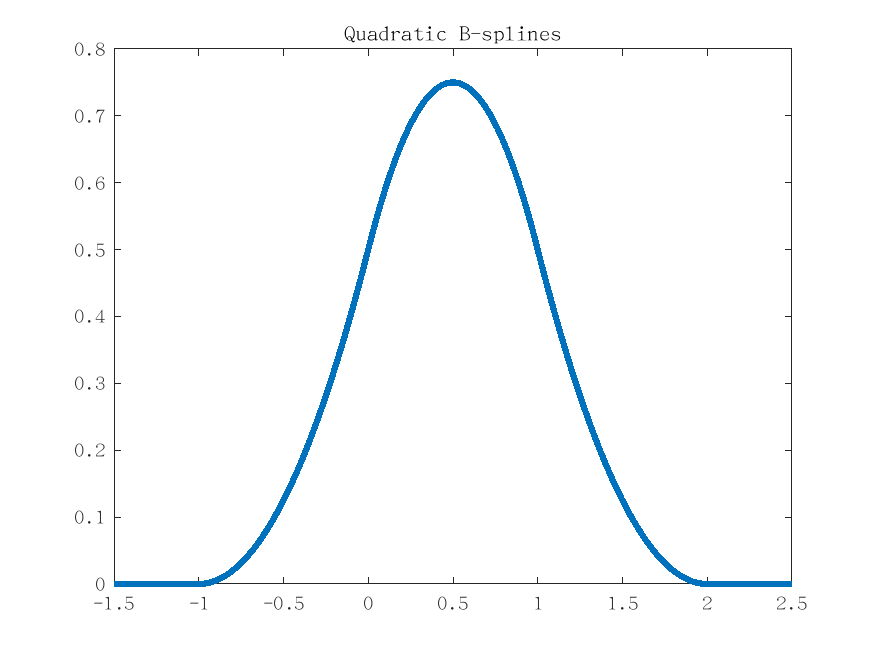
\includegraphics[width=0.8\textwidth]{QuadBspline.png}

  \lstset{language=Matlab}
  \begin{lstlisting}
  %This is a file named plotHW35.m.
    figure(1);
    x=-1.5:0.01:2.5;
    y=0.5.*((x+1).^2).*(x>=-1 & x<=0)+(0.5.*(x+1).*(1-x)+0.5.*(2-x).*x).*(x>0 & x <=1)+ 0.5.*((2-x).^2).*(x>1 & x<=2);
    plot(x,y,'LineWidth',3);
    title('Quadratic B-splines');
    saveas(1,'QuadBspline.png');
  \end{lstlisting}
\end{proof}

\RNum{6}.
\begin{proof}
  \begin{align*}
    &(t_{i+2}-t_{i-1})[t_{i-1},t_i,t_{i+1},t_{i+2}](t-x)^2_+\\
    =&[t_i,t_{i+1},t_{i+2}](t-x)^2_+ - [t_{i-1},t_i,t_{i+1}](t-x)^2_+\\
    =&(t_i-x)[t_i,t_{i+1},t_{i+2}](t-x)_+ + [t_{i+1},t_{i+2}](t-x)_+ 
    - (t_{i-1}-x)[t_{i-1},t_i,t_{i+1}](t-x)_+ - [t_i,t_{i+1}](t-x)_+ \\
    =&\frac{t_i-x}{t_{i+2}-t_i}B^1_{i+1} - \frac{t_{i-1}-x}{t_{i+1}-t_{i-1}}B^1_{i}+([t_{i+1},t_{i+2}](t-x)_+-[t_i,t_{i+1}](t-x)_+)\\
    =&\frac{t_i-x}{t_{i+2}-t_i}B^1_{i+1} - \frac{t_{i-1}-x}{t_{i+1}-t_{i-1}}B^1_{i}+\frac{[t_{i},t_{i+1},t_{i+2}](t-x)_+}{t_{i+2}-t_{i}}\\
    =&\frac{t_i-x}{t_{i+2}-t_i}B^1_{i+1} - \frac{t_{i-1}-x}{t_{i+1}-t_{i-1}}B^1_{i}+\frac{t_{i+2}-t_i}{t_{i+2}-t_{i}}B^1_{i+1}\\
    =&\frac{t_{i+2}-x}{t_{i+2}-t_i}B^1_{i+1} + \frac{x-t_{i-1}}{t_{i+1}-t_{i-1}}B^1_{i}\\
    =&B^2_i,
  \end{align*}
  where the second step follows from (4.37), the third and fifth from Example 4.32.
\end{proof}

\RNum{7}
\begin{proof}
  By Theorem on derivatives of B-splines, we have 
  \begin{align*}
    \difFrac{}{x}B^{n+1}_i(x)=(n+1)(\frac{B^n_i(x)}{t_{i+n}-t_{i-1}}-\frac{B^n_{i+1}(x)}{t_{i+1+n}-t_{i}}).
  \end{align*}
  Since $ \difFrac{}{x}B^{n+1}_i(x)$ is continuous, applying Newton-Leibniz formula to the LHS yields
  \begin{align*}
    \int_{t_{i-1}}^{t_{i+n+1}}\difFrac{}{x}B^{n+1}_i(x)=B^{n+1}_i(t_{i+n+1})-B^{n+1}_i(t_{i-1})=0,
  \end{align*}
  which means RHS's integral along $[t_{i-1},t_{i+n+1}]$ also equals 0, i.e. 
  \begin{align*}
    \int_{t_{i-1}}^{t_{i+n+1}}(\frac{B^n_i(x)}{t_{i+n}-t_{i-1}}-\frac{B^n_{i+1}(x)}{t_{i+1+n}-t_{i}})dx= 0.
  \end{align*}
  Since the interval of support of $B^n_i$ is $[t_{i-1},t_n]$, we have 
  \begin{align*}
    \int_{t_{i-1}}^{t_{i+n}}\frac{B^n_i(x)}{t_{i+n}-t_{i-1}}dx=\int_{t_{i}}^{t_{i+n+1}}\frac{B^n_{i+1}(x)}{t_{i+1+n}-t_{i}}dx,    
  \end{align*}
  which implies for all $i$, the scaled integral of the B-spline equals to each other, 
  even if the spacing of the knots is not uniform.
\end{proof}

\RNum{8}
\begin{proof}
  For (a), when $m=4,n=2$ we have 
\begin{align*}
  \begin{array}{c|ccc}x_i&x_i^4&&\\x_{i+1}&x_{i+1}^4&(x_{i+1}+x_i)(x_i^2+x_{i+1}^2)&\\x_{i+2}&x_{i+2}^4&(x_{i+2}+x_{i+1})(x_{i+1}^2+x_{i+2}^2)&K\end{array}
\end{align*}
where 
\begin{align*}
  K&=\frac{(x_{i+2}+x_{i+1})(x_{i+2}^2+x_{i+1}^2)-(x_{i+1}+x_{i})(x_{i+1}^2+x_{i}^2)}{x_{i+2}-x_i}\\
  &=\frac{x_{i+2}^3-x_i^3+x_{i+1}^2(x_{i+2}-x_i)+x_{i+1}(x_{i+2}^2-x_i^2)}{x_{i+2}-x_i}\\
  &=x_{i+2}^2+x_i^2+x_{i+2}x_i+x_{i+1}^2+x_{i+1}(x_{i+2}+x_{i})\\
  &=\tau_2(x_i,x_{i+1},x_{i+2}). 
\end{align*}

For (b), the proof is an induction on $n$ by inverse order. 
For $n=m$, (4.55) reduces to 
\[
\tau_0(x_i,\cdots,x_{i+m})=[x_i,\cdots,x_{i+m}]x^m.  
\]
By definition, LHS = 1. Also, the m-th order derivative of 
$x^m$ is constant and equals $m!$ . Then apply Corollary 3.22 and RHS equals $m!/m!=1$, 
which proves this case. Now suppose (4.55) holds for a non-negative integer (n+1), 
with $n+1<m$. Next we will show (4.55) also holds for $n$. We have  
\begin{align*}
  \tau_{m-n}(x_i,\cdots,x_{i+n})&= \tau_{m-n}(x_i,\cdots,x_{i+n+1})-x_{i+n+1}\tau_{m-n-1}(x_i,\cdots,x_{i+n+1})\\
  &=\tau_{(m+1)-(n+1)}(x_i,\cdots,x_{i+n+1})-x_{i+n+1}\tau_{m-(n+1)}(x_i,\cdots,x_{i+n+1})\\
  &=[x_i,\cdots,x_{i+n+1}]x^{m+1}-x_{i+n+1}[x_i,\cdots,x_{i+n+1}]x^{m}\\
  &=[x_i,\cdots,x_{i+n+1}](x^{m}x)-x_{i+n+1}[x_i,\cdots,x_{i+n+1}]x^{m}\\
  &=[x_i,\cdots,x_{i+n}]x^{m},
\end{align*}
where the first step follows from the lemma on the recursive relation on complete symmetric 
polynomials, the third step from the induction hypothesis, the fifth step from Leibniz formula 
for divided difference and a simple fact that 
\begin{align*}
  \lbrack x_k,\cdots,x_{i+n+1}\rbrack x=\left\{\begin{array}{lc}x_{i+n+1}&k=i+n+1\\1&k=i+n\\0&i\leqslant k\leqslant i+n-1\end{array}\right.
\end{align*}
This shows the theorem is true for $n$, and so the theorem is true for all non-negative $n(\leq m)$ by mathematical induction.
\end{proof}

\section{C++ programming}
Follow the $\textbf{readme}$, and generate all answers! 
Codes are contained in the e-mail tar, and only conclusions will be shown in the following part.

\subsection{\textbf{Structure of codes}}
$\textbf{bin}$ stores compiled files;\\
$\textbf{doc}$ stores the same document as this one;\\
$\textbf{include}$ stores sources files that support spline implementation;\\
$\textbf{main}$ stores files concerning the assignments;\\
$\textbf{output}$ stores all results such as $\textbf{*.m}$ and $\textbf{*.png}$.\\
$\textbf{test}$ stores test files.\\
Results for each part are shown below, generating from $ \textbf{make runAssignment} $ and $ \textbf{make plotAssignment} $.
\subsection{\textbf{Assignment B}}
\lstset{language=C++}
\begin{lstlisting}
  ------------------------Assignment B--------------------------
  For Complete situation, 
  N = 6, error_max = 0.421705, convergence rate = 5.35038
  N = 11, error_max = 0.0103367, convergence rate = 2.16165
  N = 21, error_max = 0.00231026, convergence rate = 3.06868
  N = 41, error_max = 0.000275356, convergence rate = 4.09706
  N = 81, error_max = 1.609e-05
  For Not_a_knot situation, 
  N = 6, error_max = 0.431538, convergence rate = 5.38047
  N = 11, error_max = 0.0103594, convergence rate = 2.16482
  N = 21, error_max = 0.00231026, convergence rate = 3.06869
  N = 41, error_max = 0.000275356, convergence rate = 4.09706
  N = 81, error_max = 1.609e-05
  Plots have been generated as '/output/B_[XX]Plot.m'.
\end{lstlisting}
After plotting, we have

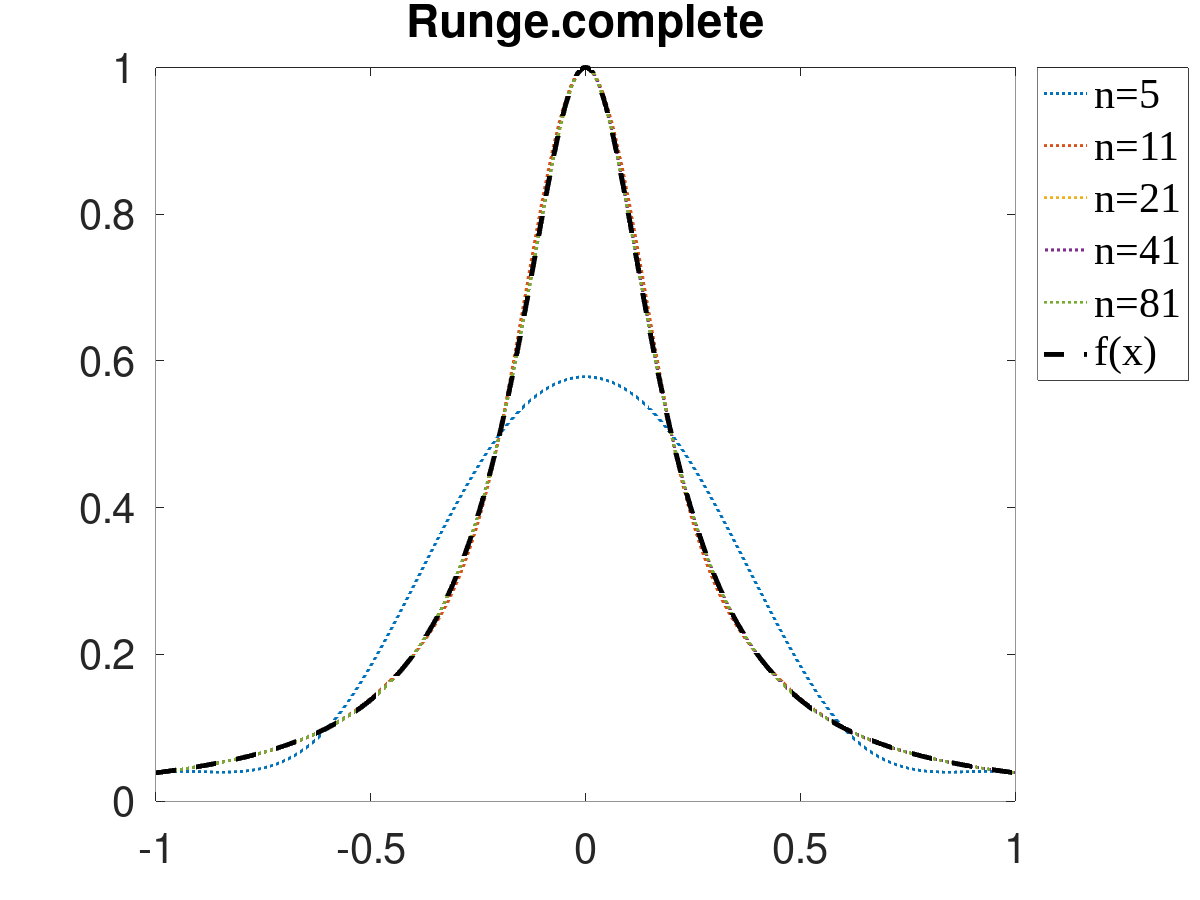
\includegraphics[width=0.45\textwidth]{figures/Assignment_B_complete.png}
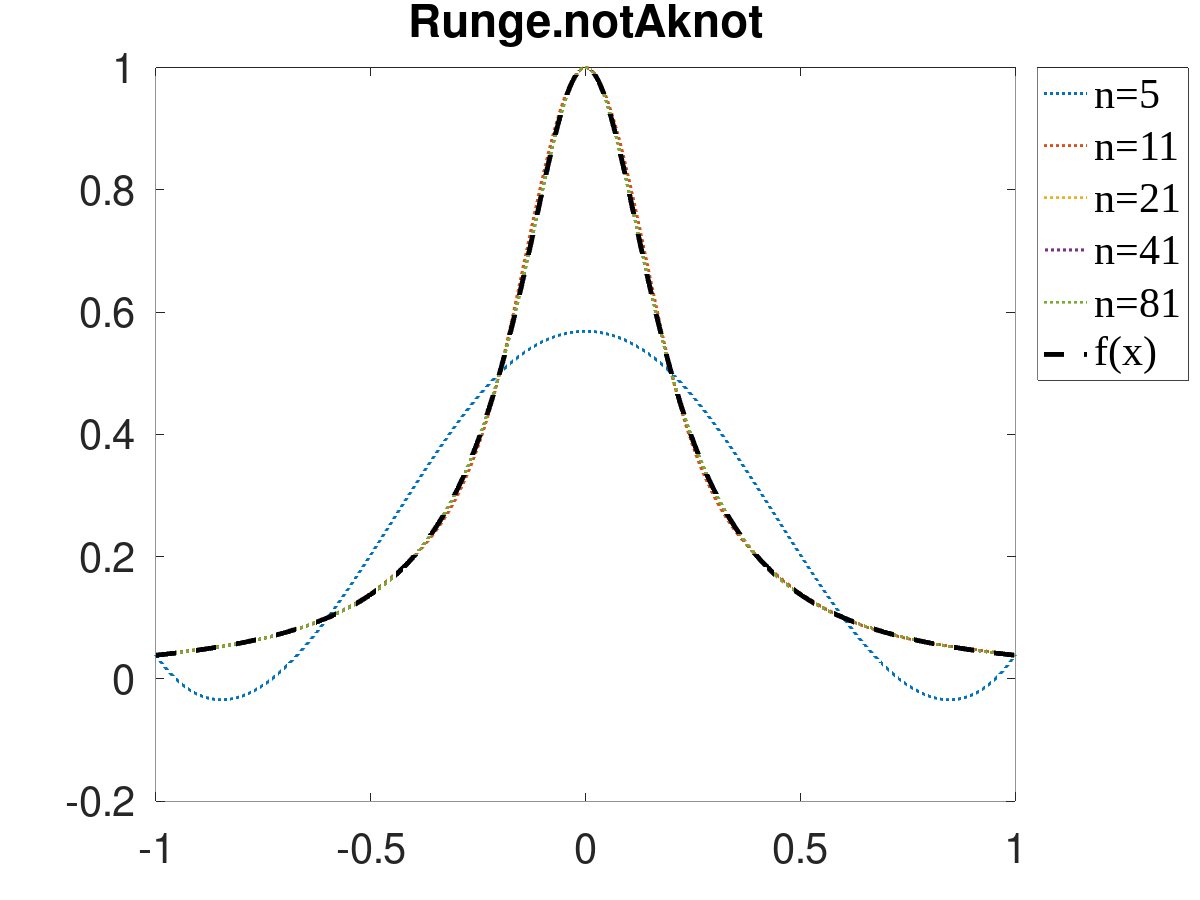
\includegraphics[width=0.45\textwidth]{figures/Assignment_B_notAknot.png}

The results show spline interpolation is indeed free of the wide oscillations in the Runge phenomenon.

\subsection*{\textbf{Assignment C and D}}
\lstset{language=C++}
\begin{lstlisting}
  ------------------------Assignment C--------------------------
  Plots have been generated as '/output/C_[XX].m'.
  ------------------------Assignment D--------------------------
  x = -3.5: E_458 = 0.000669568, E_459 = 0
  x = -3: E_458 = 0, E_459 = 0.00141838
  x = -0.5: E_458 = 0.0205289, E_459 = 1.11022e-16
  x = 0: E_458 = 1.11022e-16, E_459 = 0.120238
  x = 0.5: E_458 = 0.0205289, E_459 = 1.11022e-16
  x = 3: E_458 = 0, E_459 = 0.00141838
  x = 3.5: E_458 = 0.000669568, E_459 = 0
\end{lstlisting}
After plotting, we have

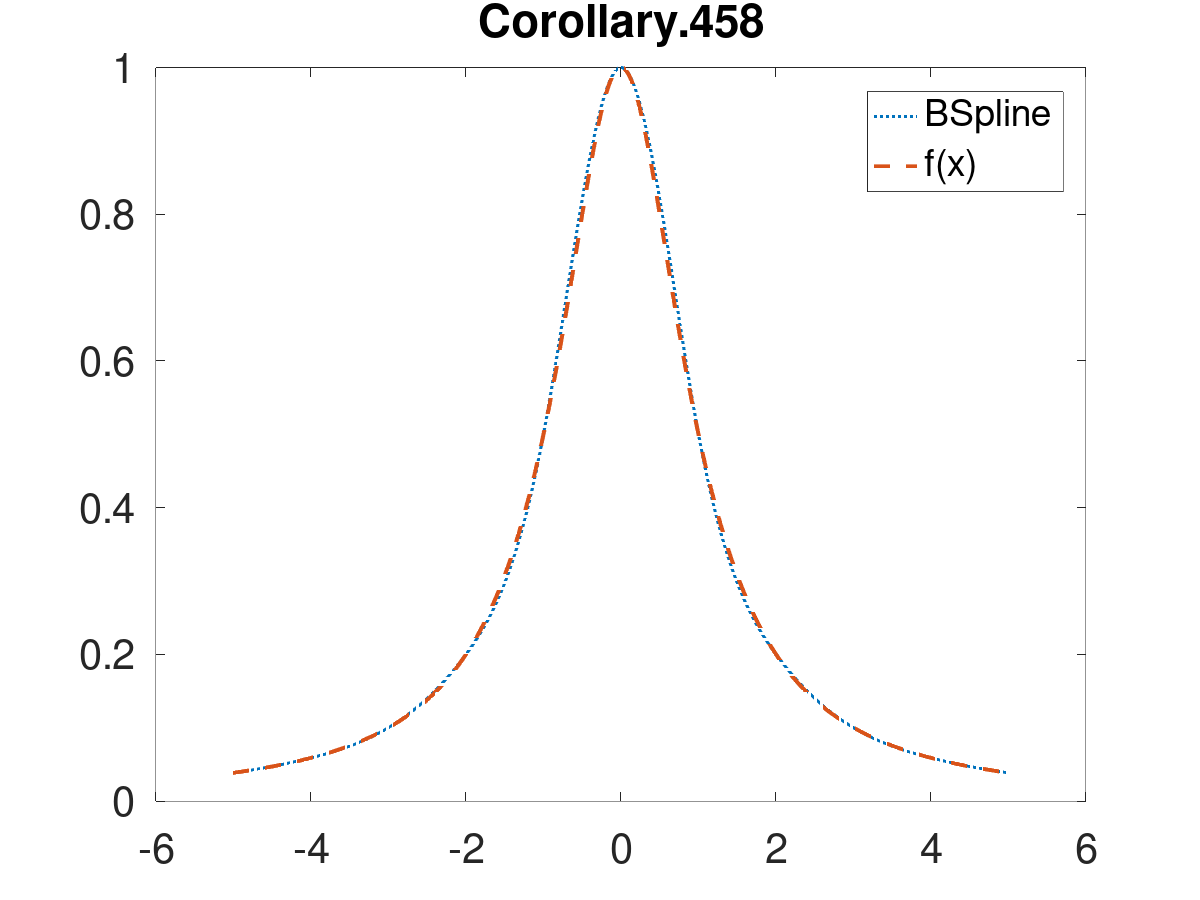
\includegraphics[width=0.45\textwidth]{figures/Assignment_C_458.png}
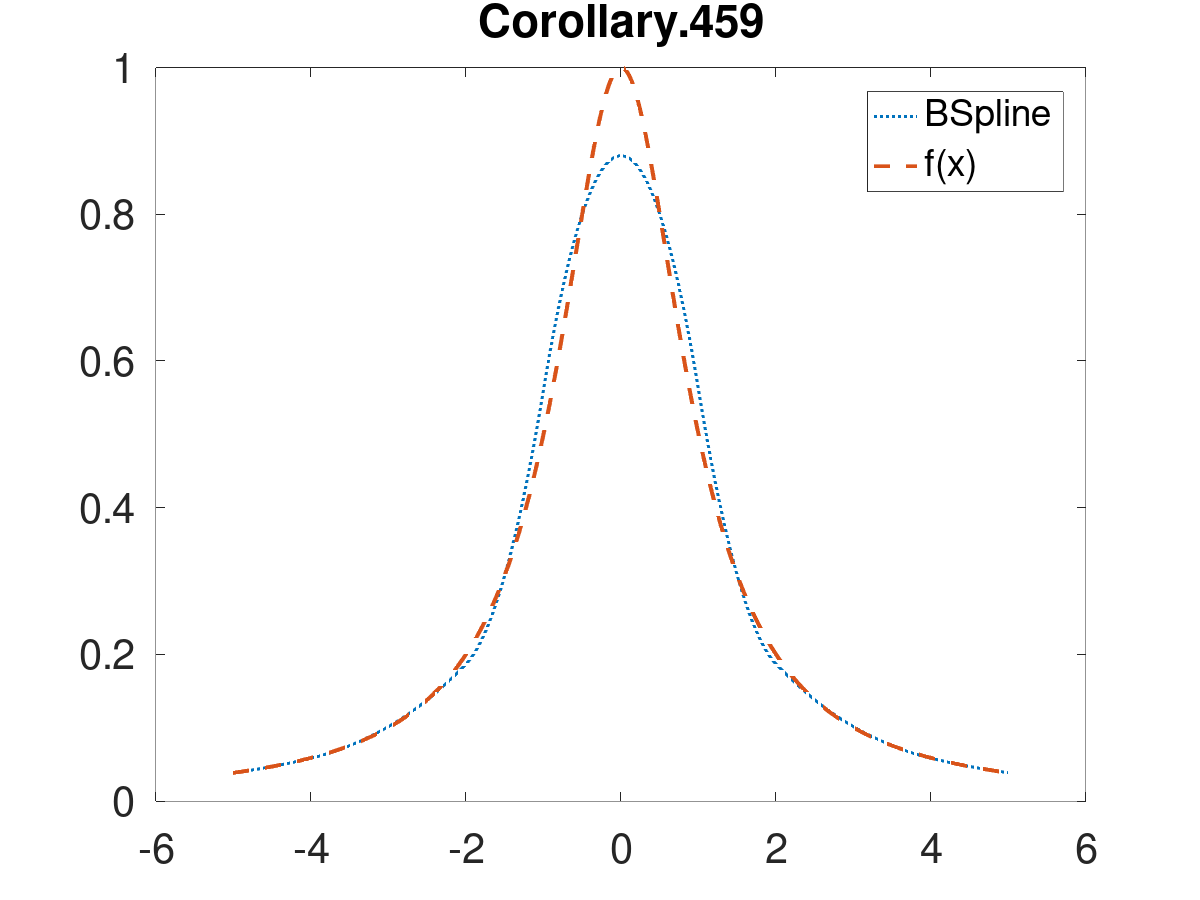
\includegraphics[width=0.45\textwidth]{figures/Assignment_C_459.png}

which answer \textbf{Assignment C}.

For \textbf{Assignment D}, it's trivial to see that the interpolation spline will have 
its error close to machine precision on its interpolation sites, since the function values 
on those points are given as preconditions and used as the RHS of linear equations that any 
solution shall satisfy. 

Also, from the maximums of middle point errors and the above plots, the first B-spline, a complete cubic 
cardinal B-spline, is more accurate.

\subsection{\textbf{Assignment E}}
\lstset{language=C++}
We apply \textbf{Spline<2,4,ppForm> fitCurve} with \textbf{BCType = periodic} since it's 
a simple close curve. 
\begin{lstlisting}
  ------------------------Assignment E--------------------------
  Plots have been generated as '/output/E_[XX].m'.
\end{lstlisting}
After plotting, we have

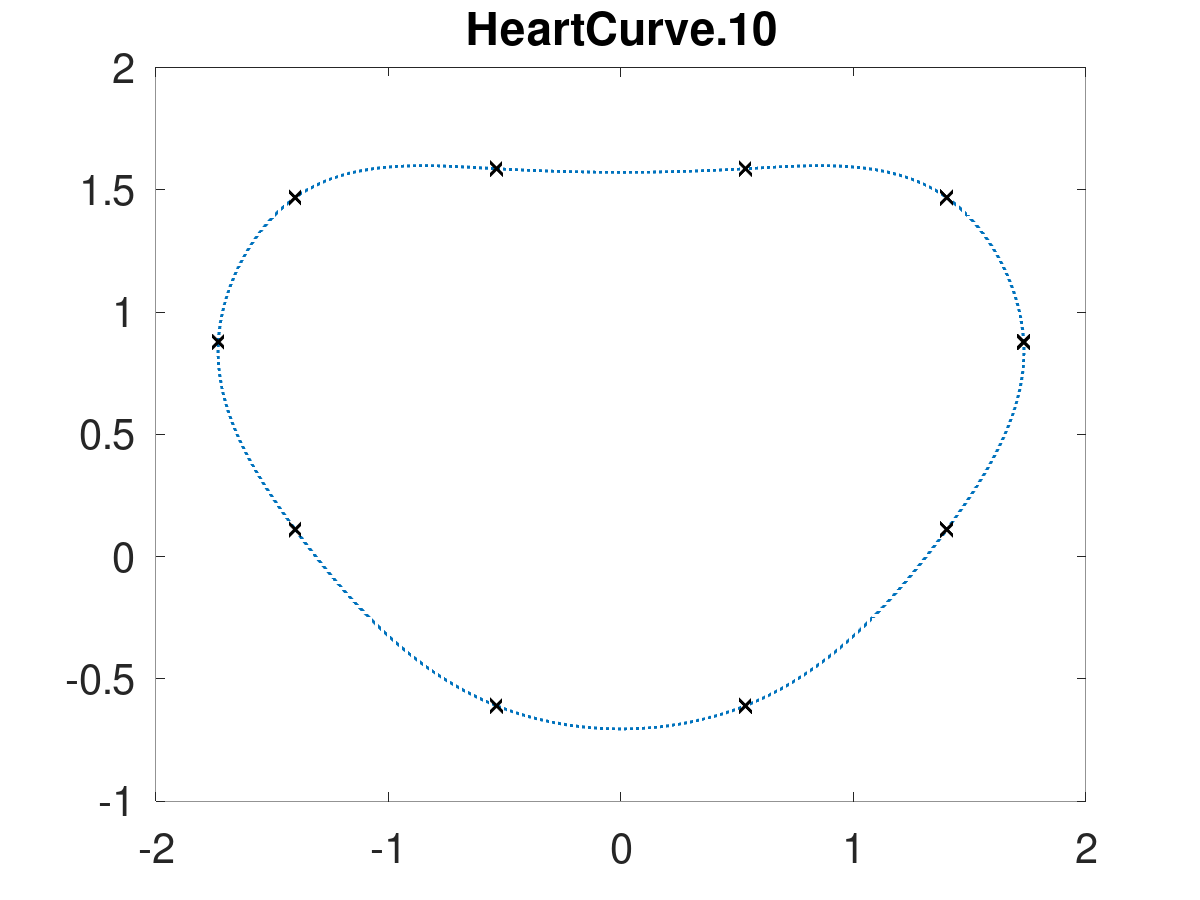
\includegraphics[width=0.45\textwidth]{figures/Assignment_E_10.png}
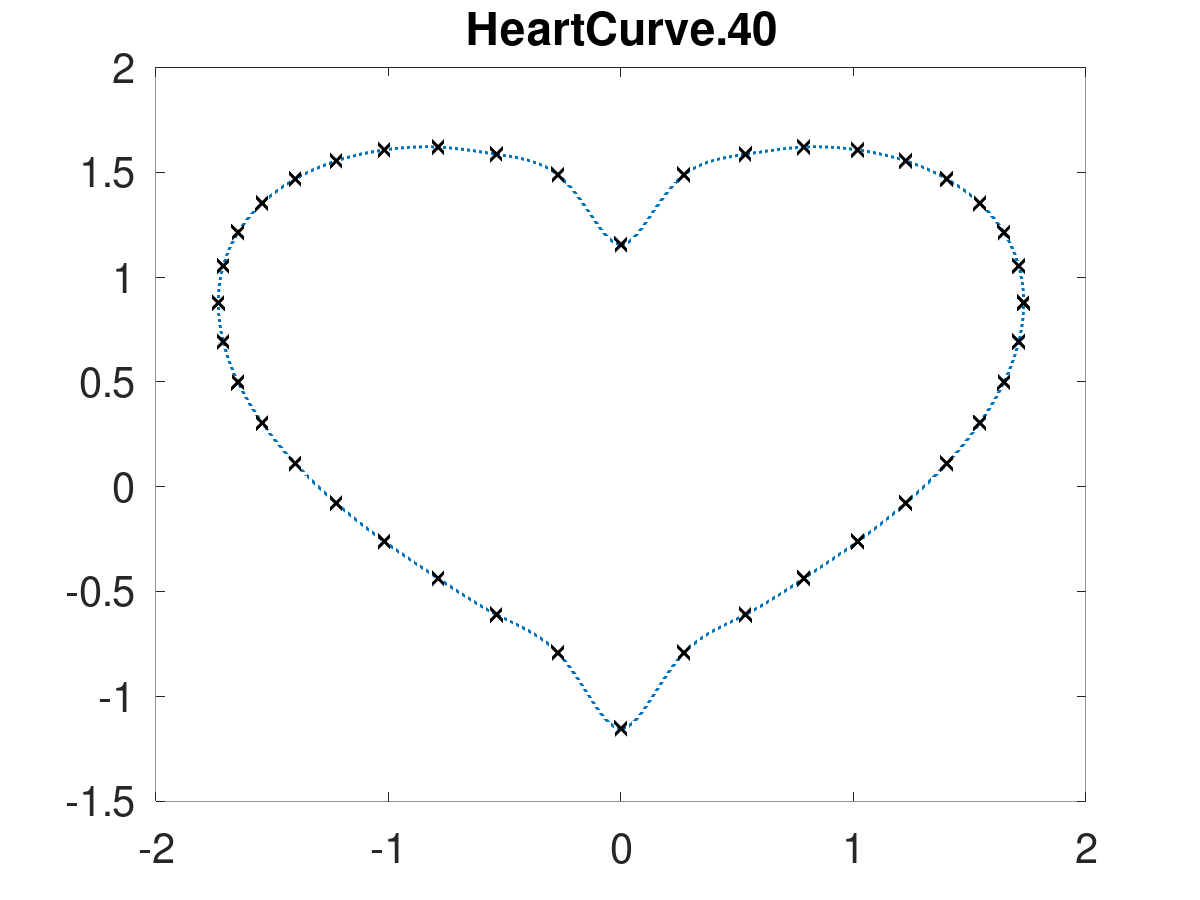
\includegraphics[width=0.45\textwidth]{figures/Assignment_E_40.png}

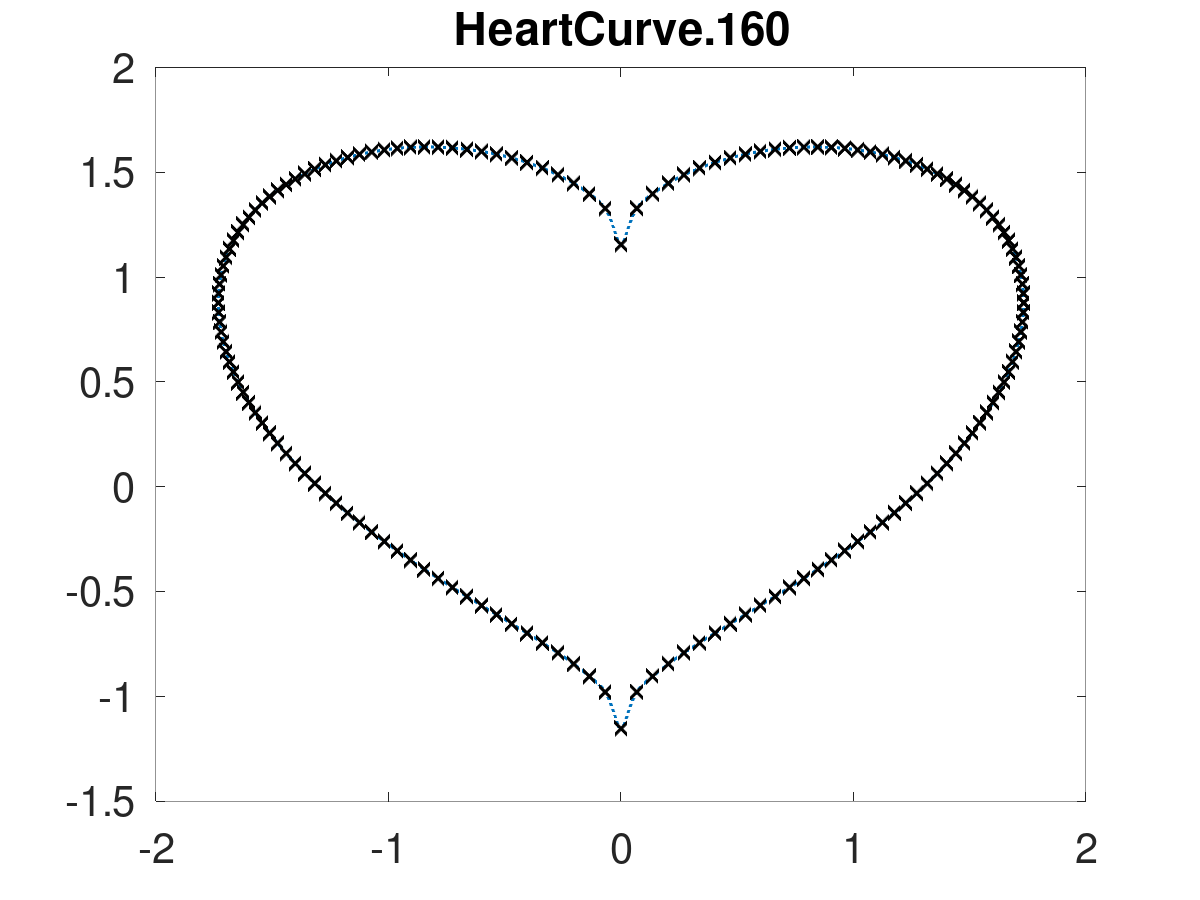
\includegraphics[width=0.5\textwidth]{figures/Assignment_E_160.png}

\subsection{\textbf{Assignment F}}
\lstset{language=C++}
\begin{lstlisting}
  ------------------------Assignment F--------------------------
  Plots have been generated as '/output/F_beastPlot.m'.
\end{lstlisting}
After plotting, we have

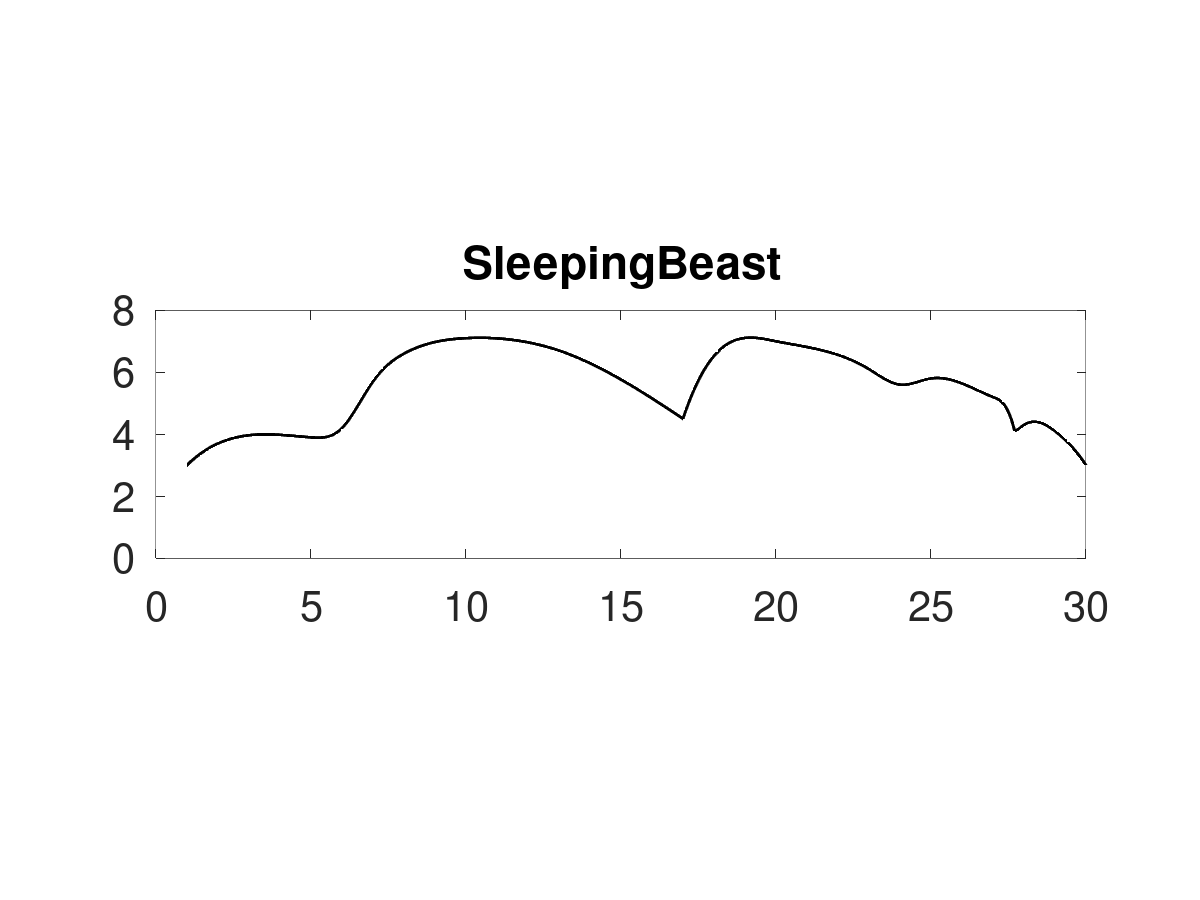
\includegraphics[width=0.5\textwidth]{figures/Assignment_F_beastPlot.png}


\subsection{\textbf{Assignment G}}
\lstset{language=C++}
\begin{lstlisting}
  ------------------------Assignment G--------------------------
  Plots have been generated as '/output/G_N[X].m'.
  
  ------------------------All Assignments Completed------------------------
\end{lstlisting}
After plotting, we have

\begin{figure}[!htbp]
  \flushleft
  \subfigure
  {
  \begin{minipage}[b]{.3\linewidth}
    \flushleft
  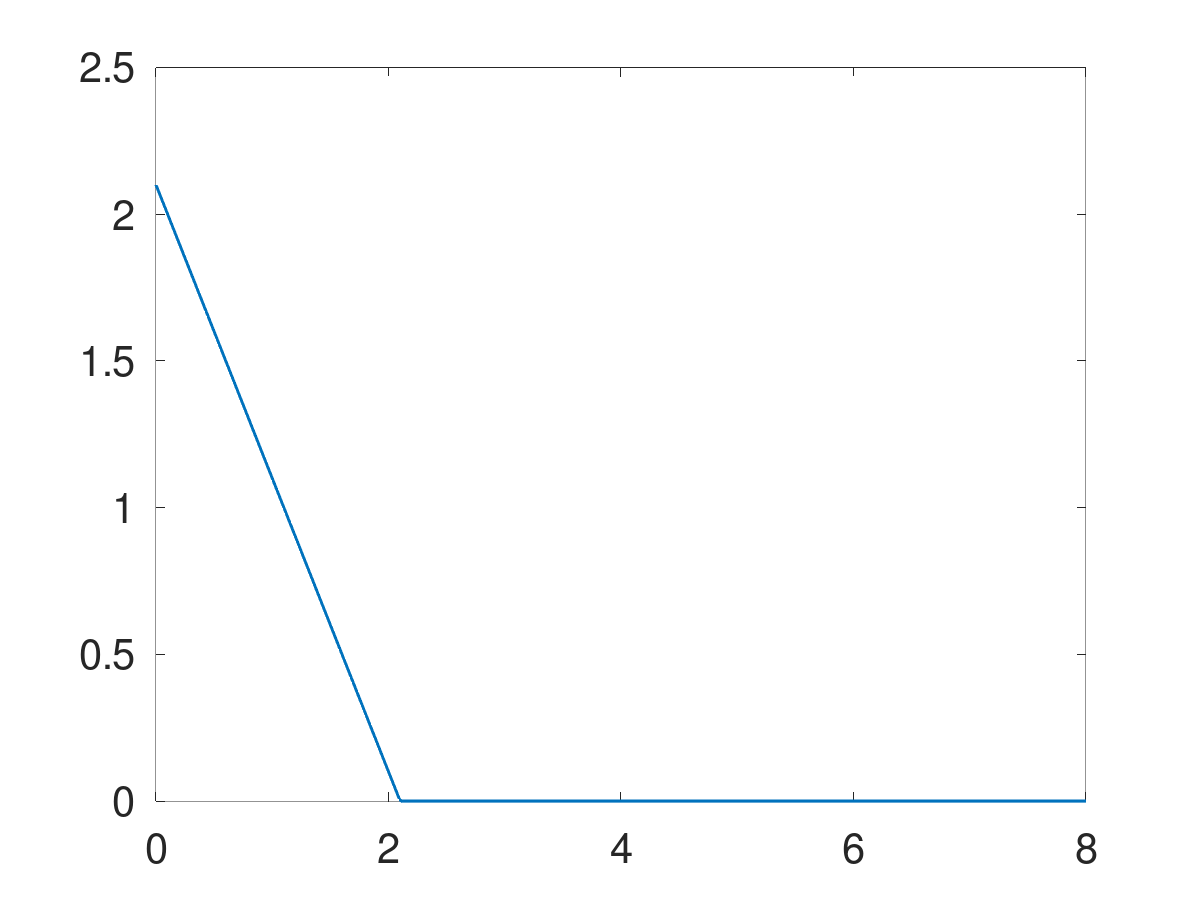
\includegraphics[scale=0.1]{figures/Assignment_G_N1_0_0.png}
  \end{minipage}
  }
  \subfigure
  {
  \begin{minipage}[b]{.3\linewidth}
    \flushleft
  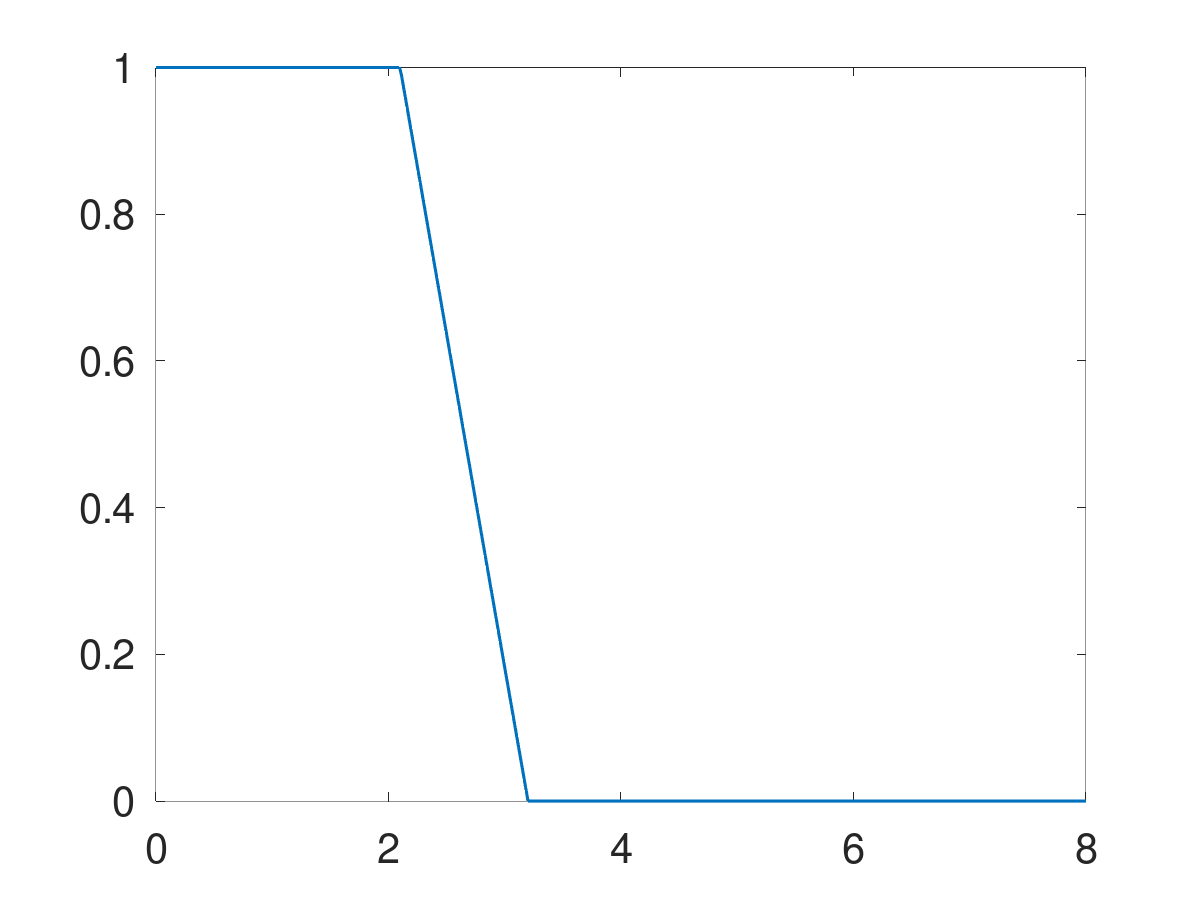
\includegraphics[scale=0.1]{figures/Assignment_G_N1_1_0.png}
  \end{minipage}
  }
  \subfigure
  {
  \begin{minipage}[b]{.3\linewidth}
    \flushleft
  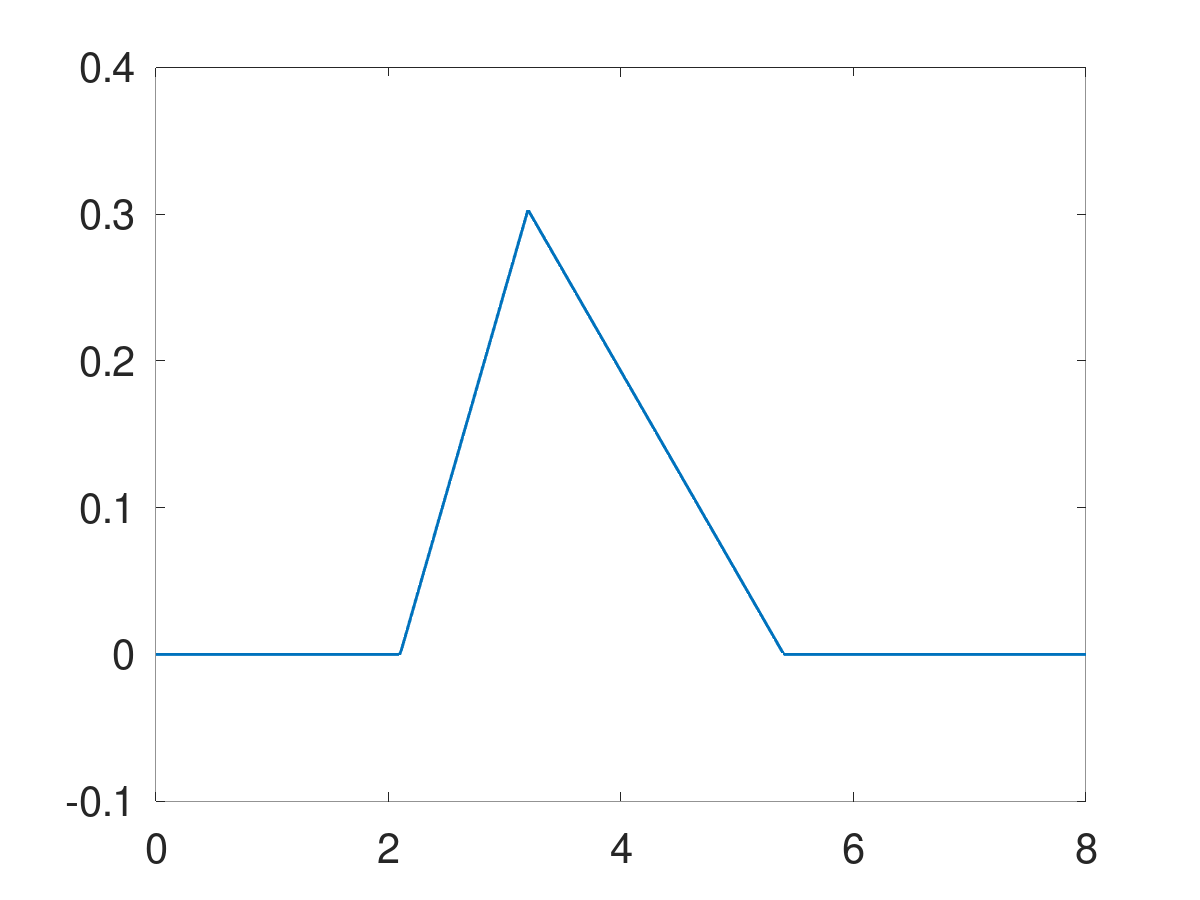
\includegraphics[scale=0.1]{figures/Assignment_G_N1_2_0.png}
  \end{minipage}
  }
  \subfigure
  {
  \begin{minipage}[b]{.3\linewidth}
    \flushleft
  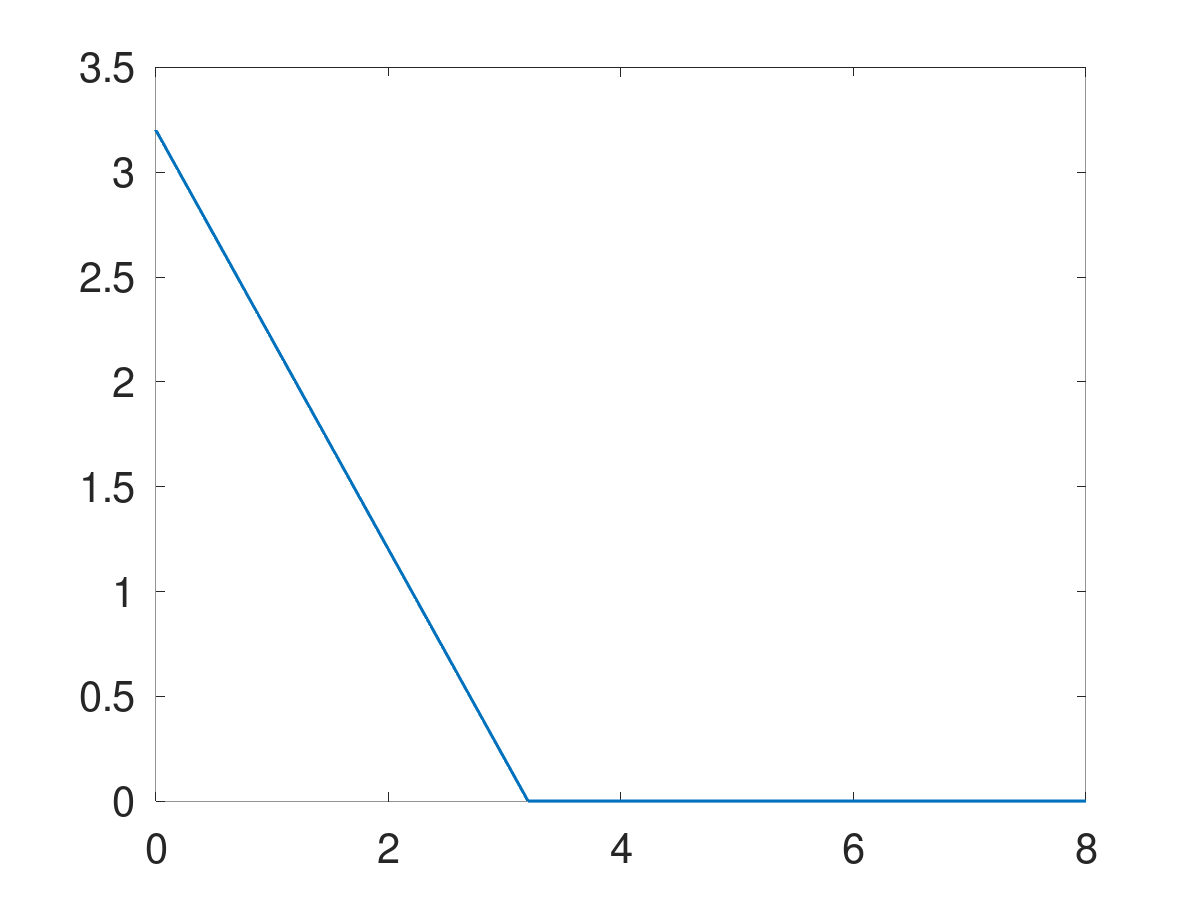
\includegraphics[scale=0.1]{figures/Assignment_G_N1_0_1.png}
  \end{minipage}
  }
  \subfigure{
  \begin{minipage}[b]{.3\linewidth}
    \flushleft
  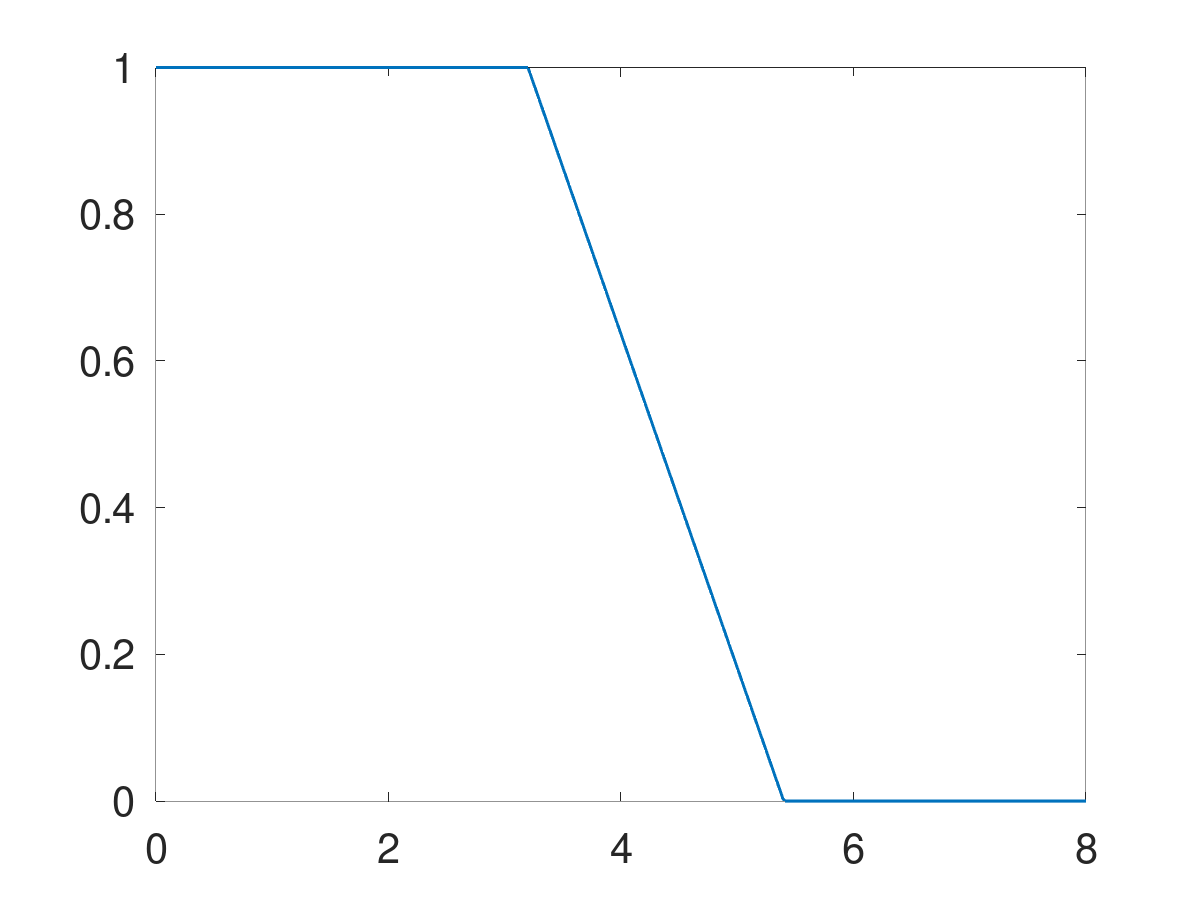
\includegraphics[scale=0.1]{figures/Assignment_G_N1_1_1.png}
  \end{minipage}
  }
  \newline
  \subfigure{
  \begin{minipage}[b]{.3\linewidth}
    \flushleft
  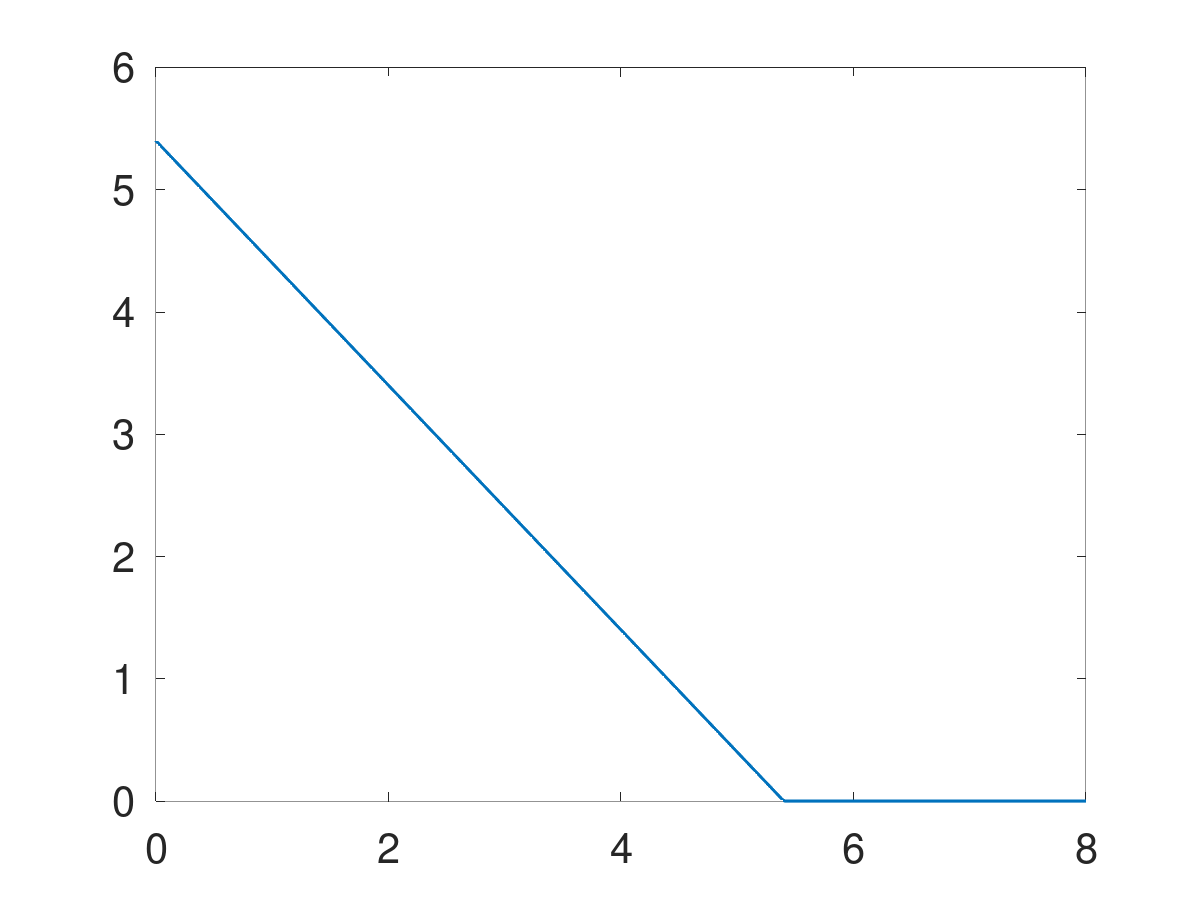
\includegraphics[scale=0.1]{figures/Assignment_G_N1_0_2.png}
  \end{minipage}
  }
  \caption{N=1}
  \end{figure}


  \begin{figure}[!htbp]
    \flushleft
    \subfigure
    {
    \begin{minipage}[b]{.23\linewidth}
      \flushleft
    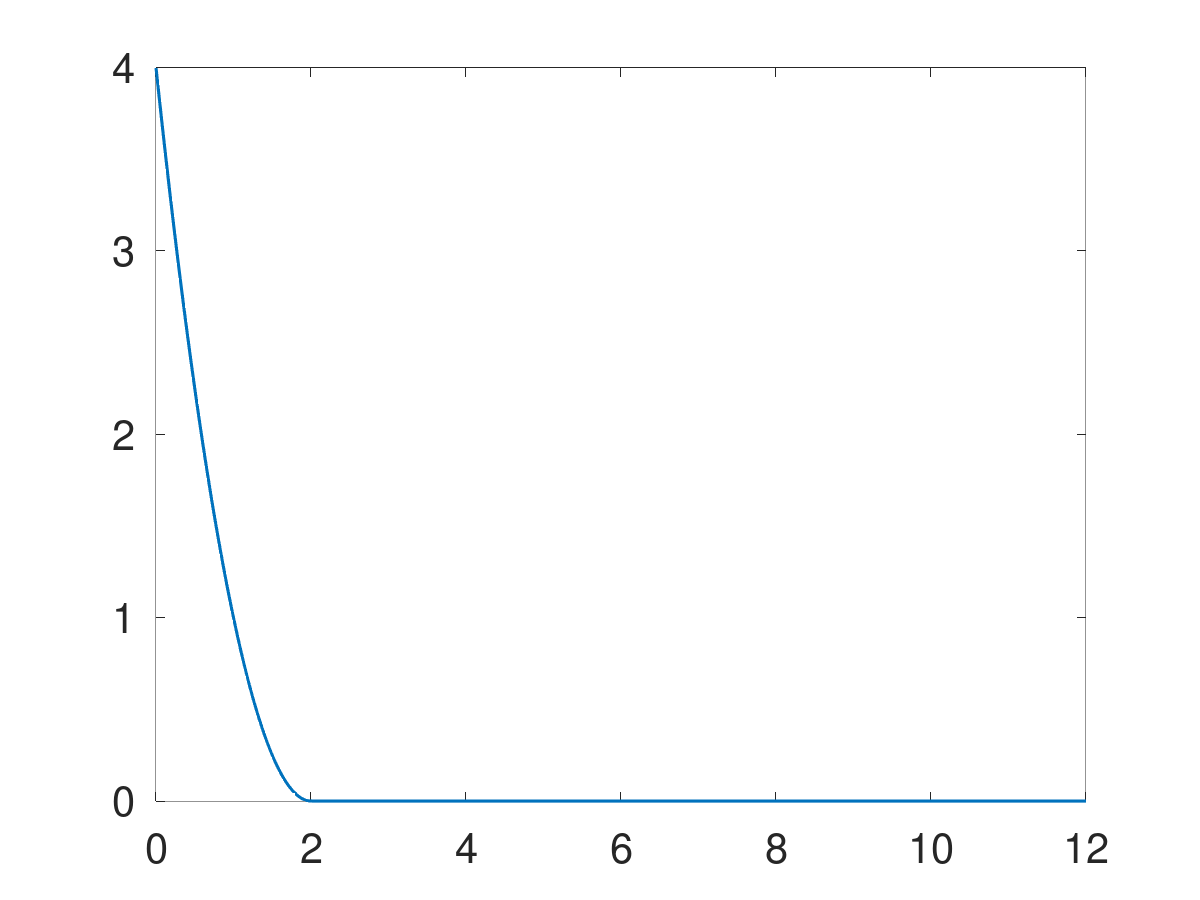
\includegraphics[scale=0.1]{figures/Assignment_G_N2_0_0.png}
    \end{minipage}
    }
    \subfigure
    {
    \begin{minipage}[b]{.23\linewidth}
      \flushleft
    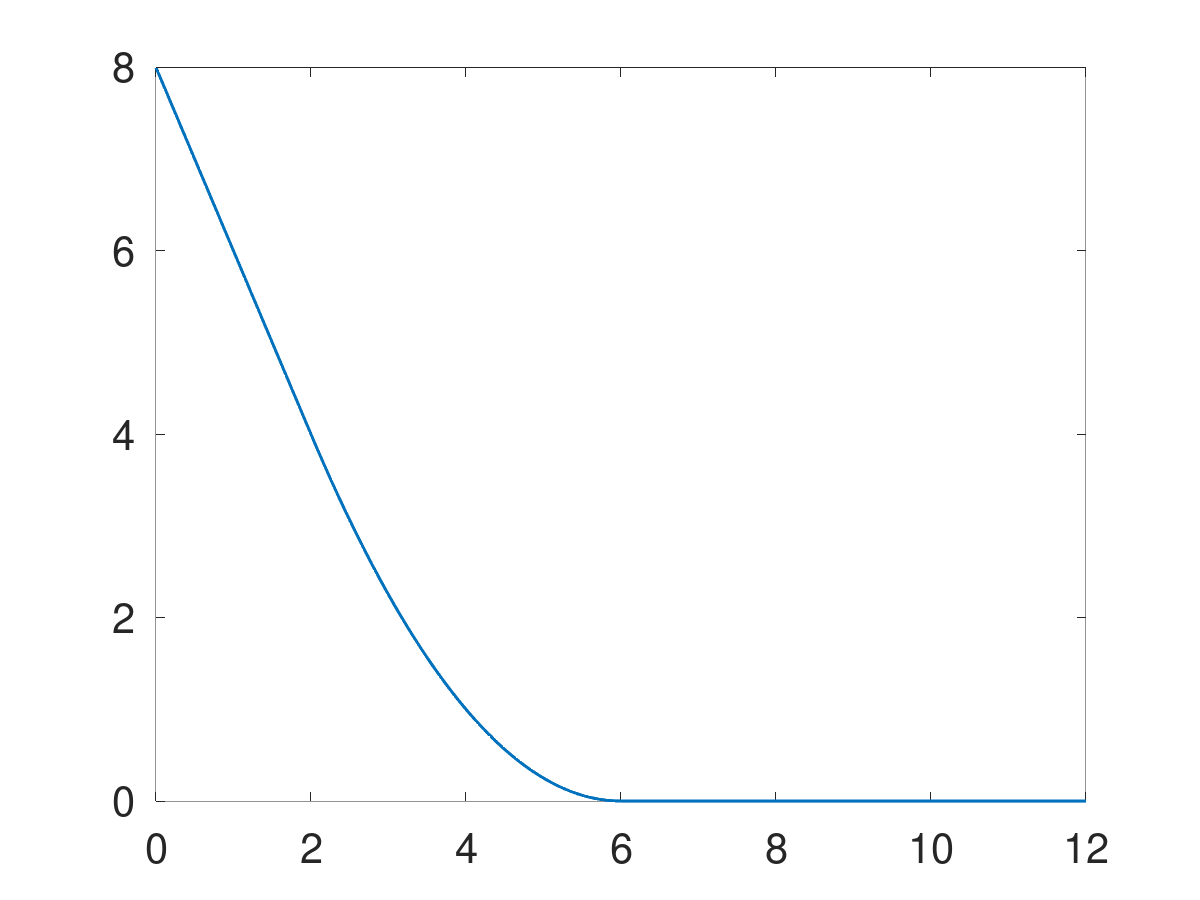
\includegraphics[scale=0.1]{figures/Assignment_G_N2_1_0.png}
    \end{minipage}
    }
    \subfigure
    {
    \begin{minipage}[b]{.23\linewidth}
      \flushleft
    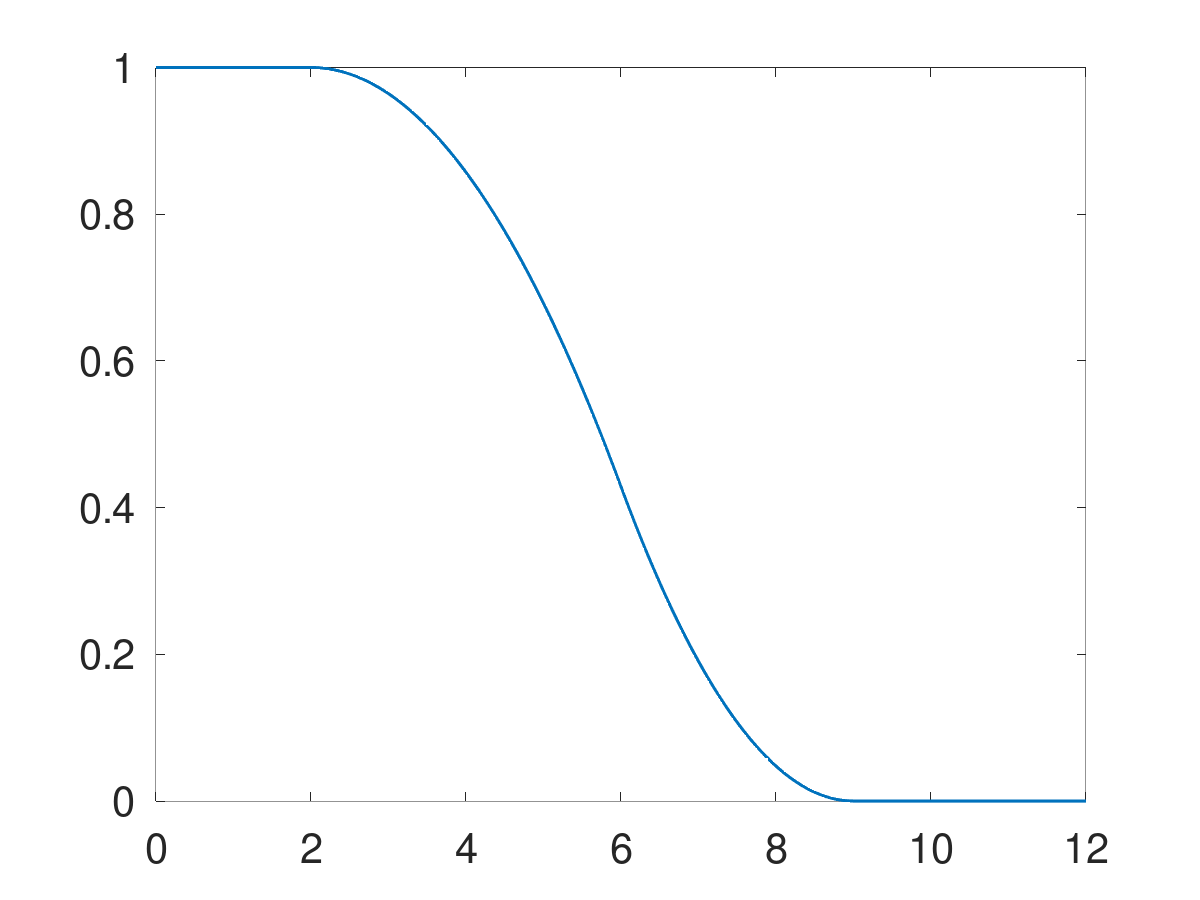
\includegraphics[scale=0.1]{figures/Assignment_G_N2_2_0.png}
    \end{minipage}
    }
    \subfigure
    {
    \begin{minipage}[b]{.23\linewidth}
      \flushleft
    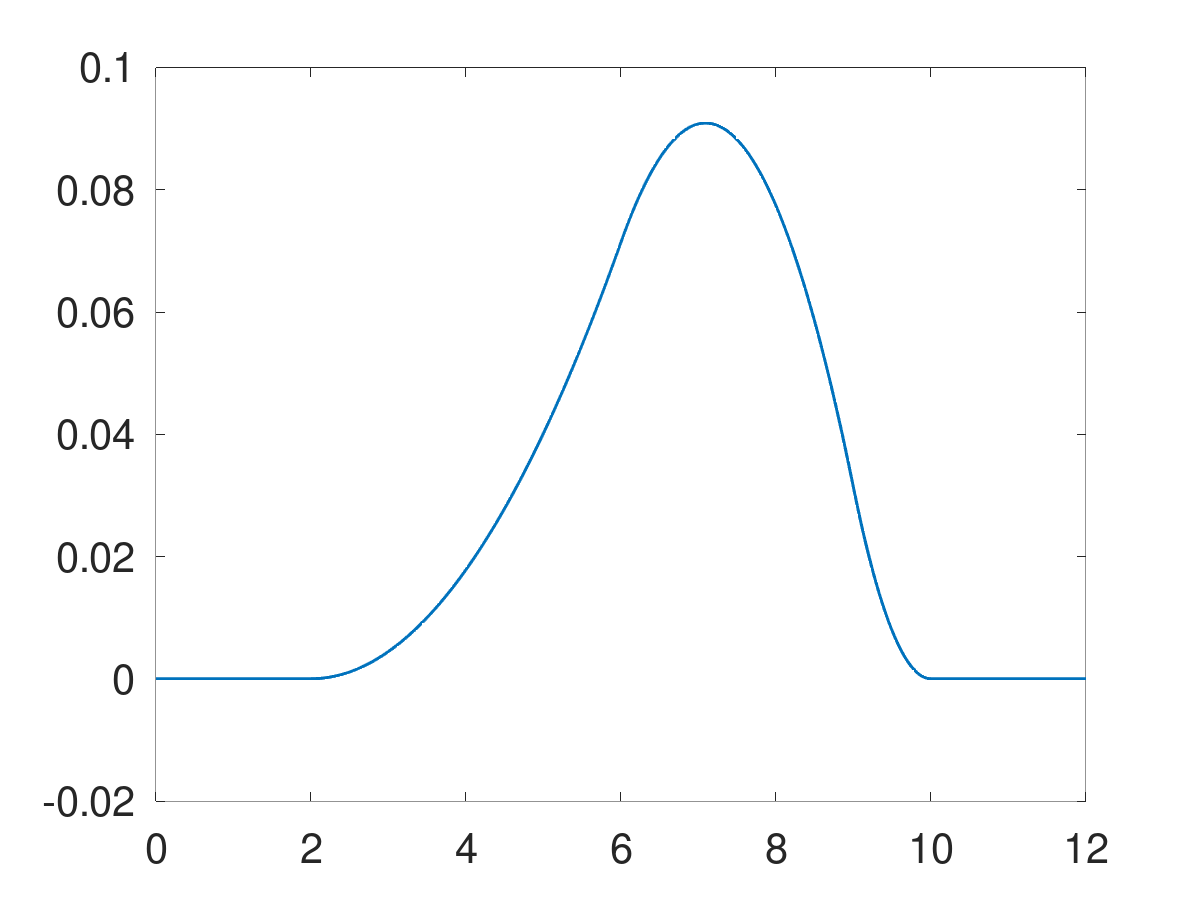
\includegraphics[scale=0.1]{figures/Assignment_G_N2_3_0.png}
    \end{minipage}
    }
    \newline
    \subfigure{
    \begin{minipage}[b]{.23\linewidth}
      \flushleft
    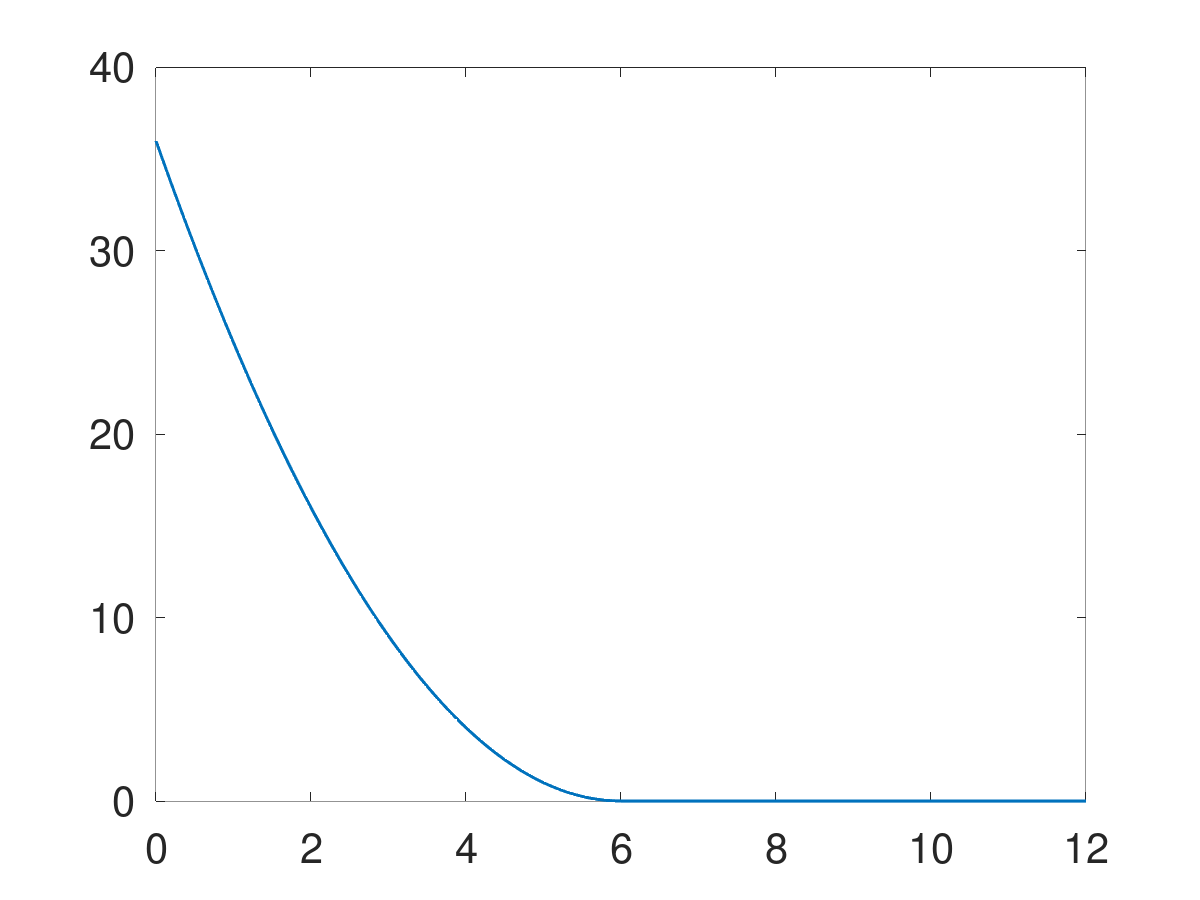
\includegraphics[scale=0.1]{figures/Assignment_G_N2_0_1.png}
    \end{minipage}
    }
    \subfigure{
    \begin{minipage}[b]{.23\linewidth}
      \flushleft
    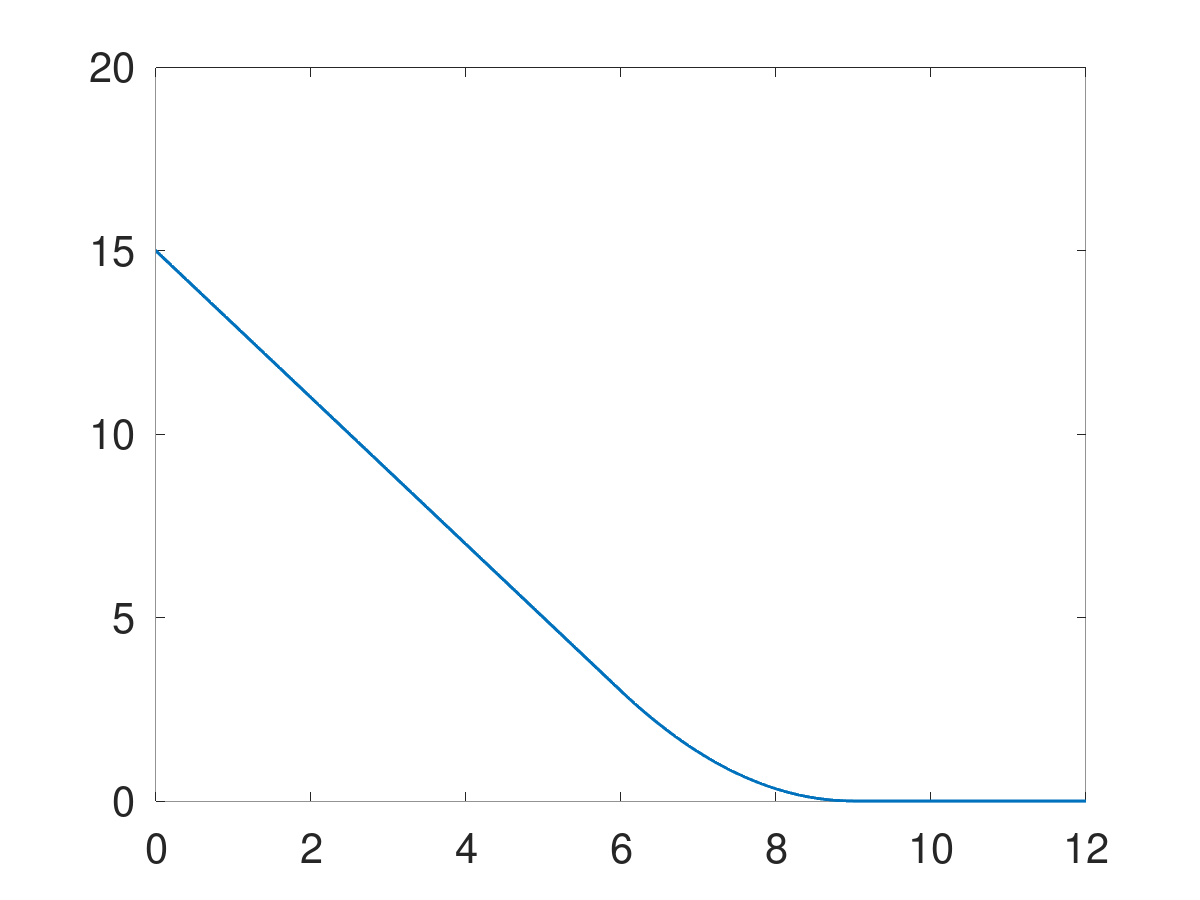
\includegraphics[scale=0.1]{figures/Assignment_G_N2_1_1.png}
    \end{minipage}
    }
    \subfigure{
      \begin{minipage}[b]{.23\linewidth}
        \flushleft
      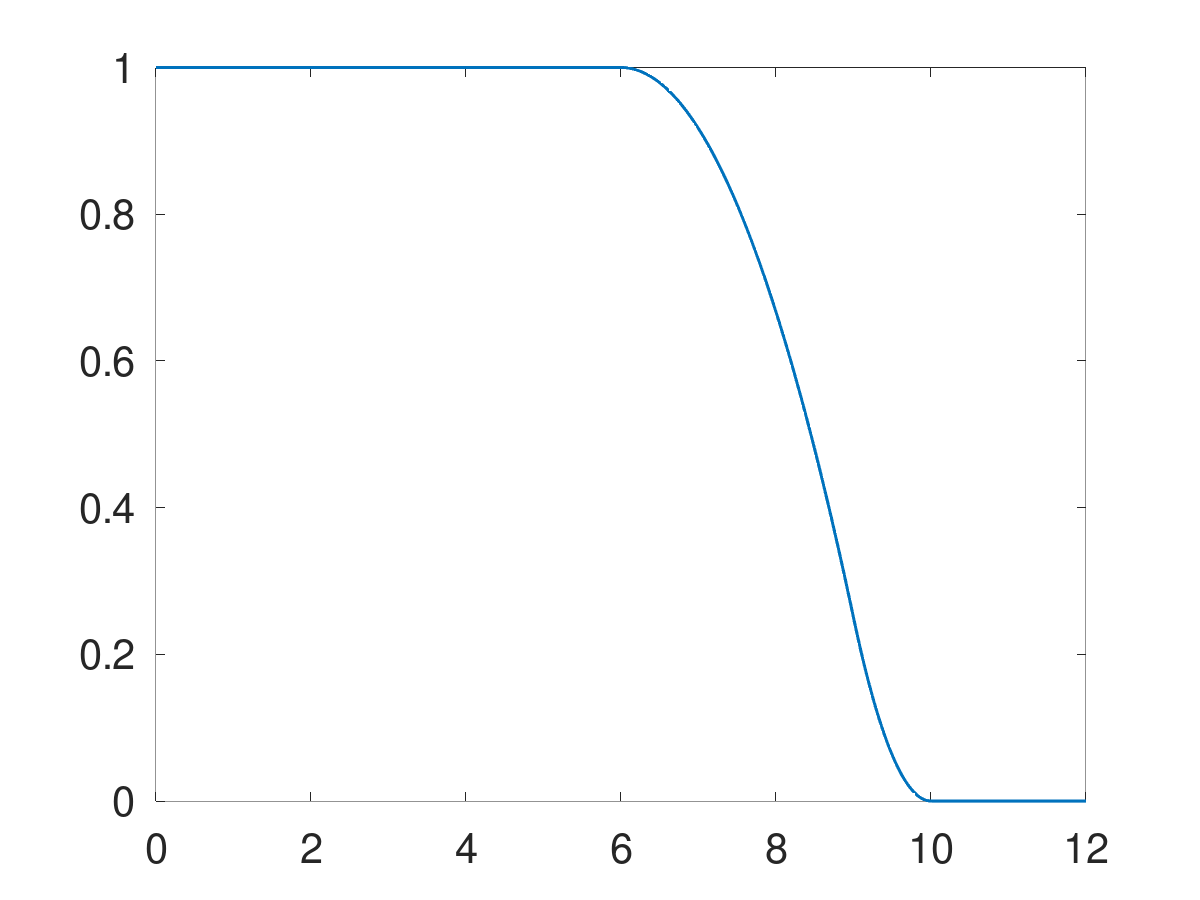
\includegraphics[scale=0.1]{figures/Assignment_G_N2_2_1.png}
      \end{minipage}
    }
    \newline
    \subfigure{
      \begin{minipage}[b]{.23\linewidth}
        \flushleft
      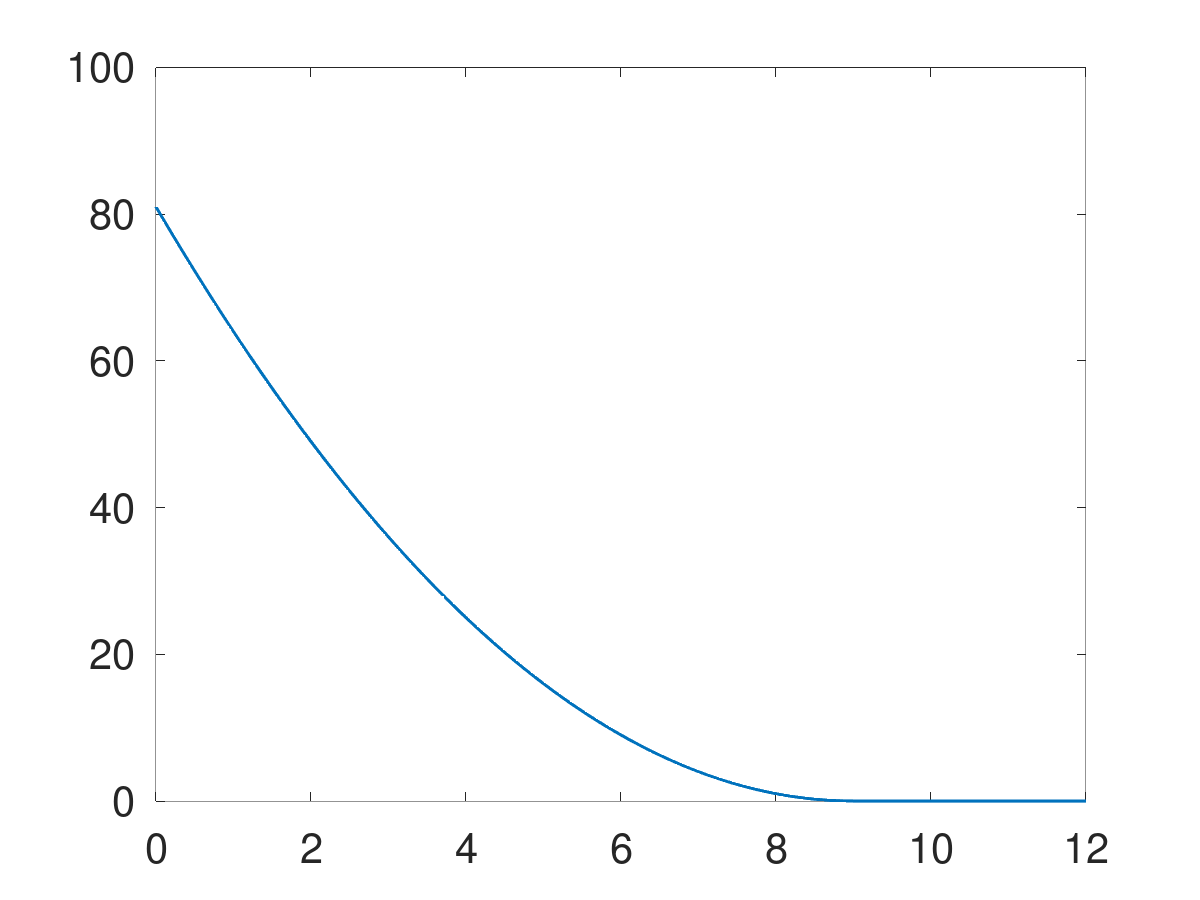
\includegraphics[scale=0.1]{figures/Assignment_G_N2_0_2.png}
      \end{minipage}
    }
    \subfigure{
    \begin{minipage}[b]{.23\linewidth}
      \flushleft
    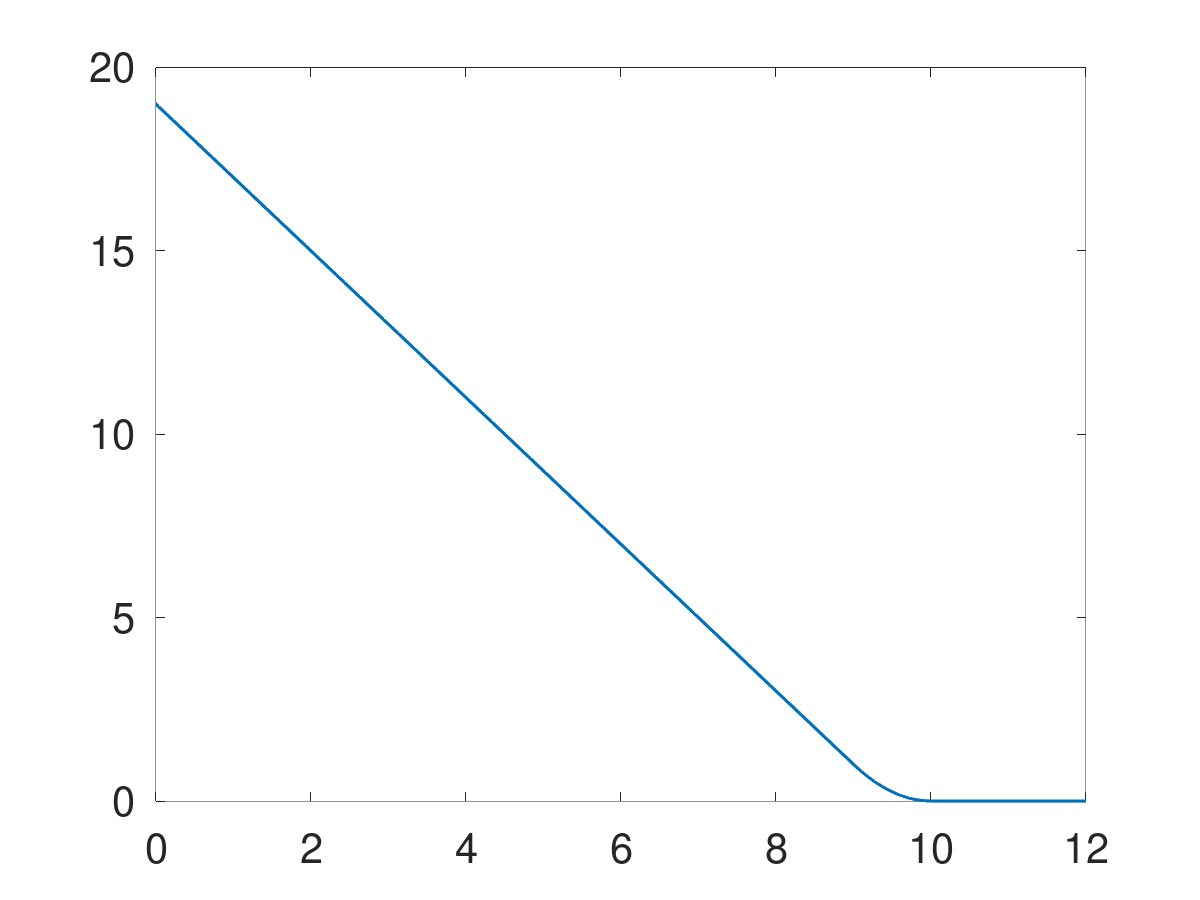
\includegraphics[scale=0.1]{figures/Assignment_G_N2_1_2.png}
    \end{minipage}
    }
    \newline
    \subfigure{
    \begin{minipage}[b]{.23\linewidth}
      \flushleft
    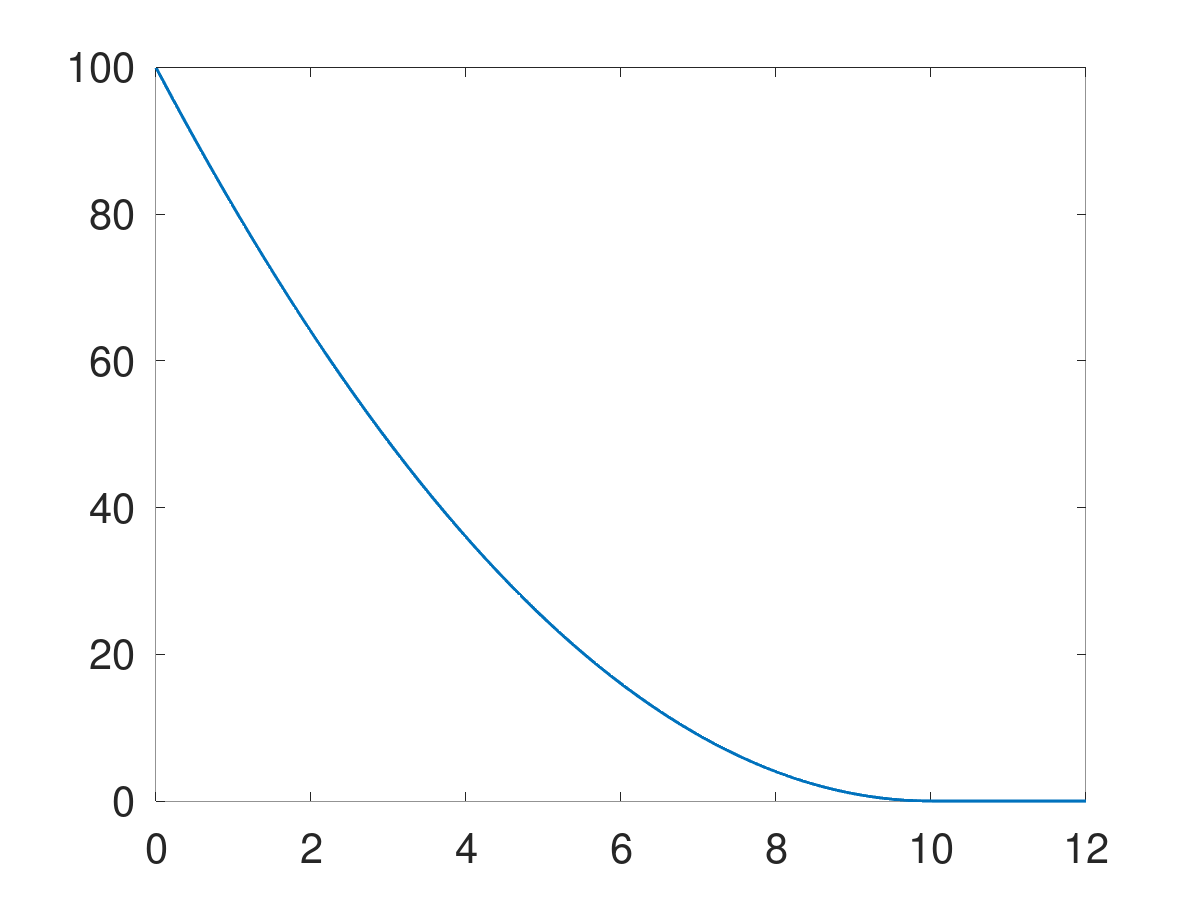
\includegraphics[scale=0.1]{figures/Assignment_G_N2_0_3.png}
    \end{minipage}
    } 
    \caption{N=2}
    \end{figure}
\newpage

    Then comparing them with B-splines that are retracted by factor $t_{i+n}-t_{i-1}$ 
    yields

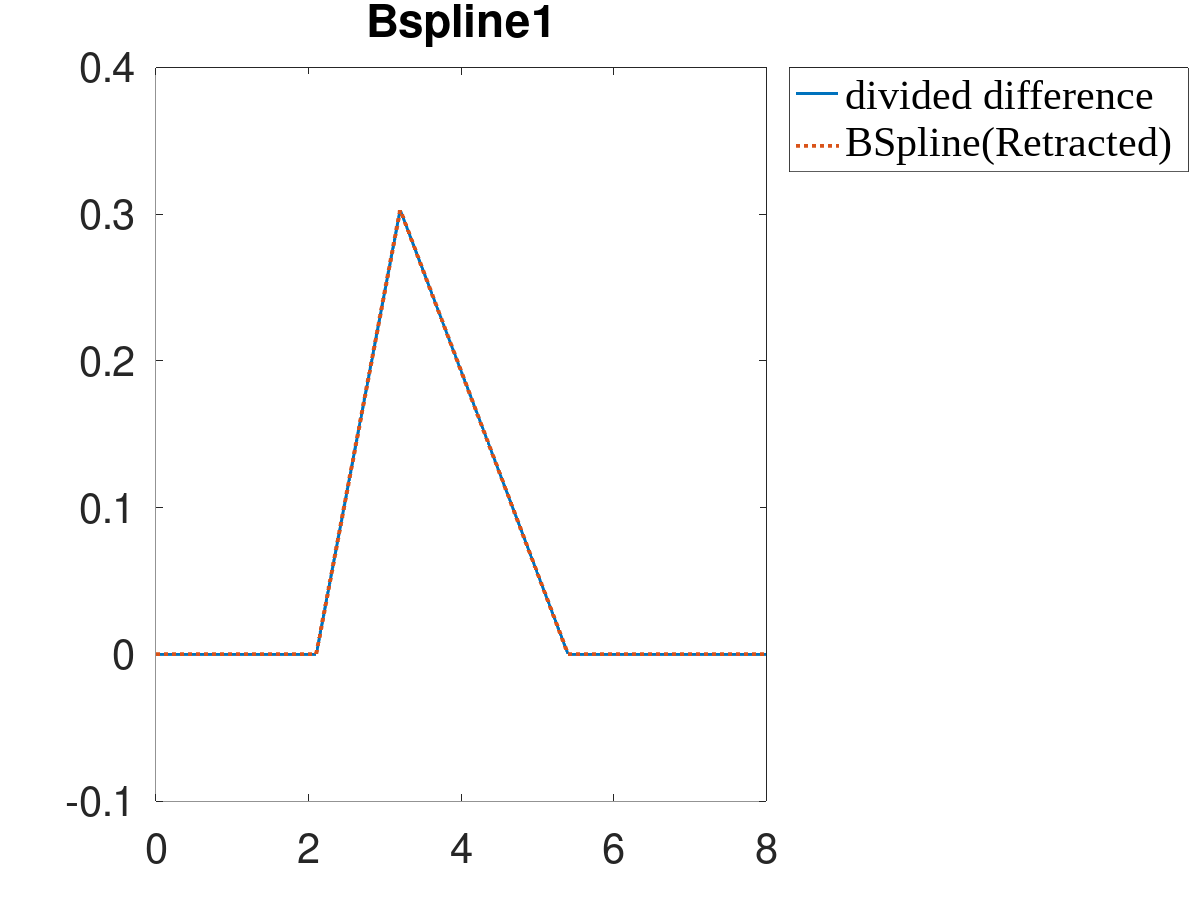
\includegraphics[width=0.45\textwidth]{figures/Assignment_G_1_Compare.png}
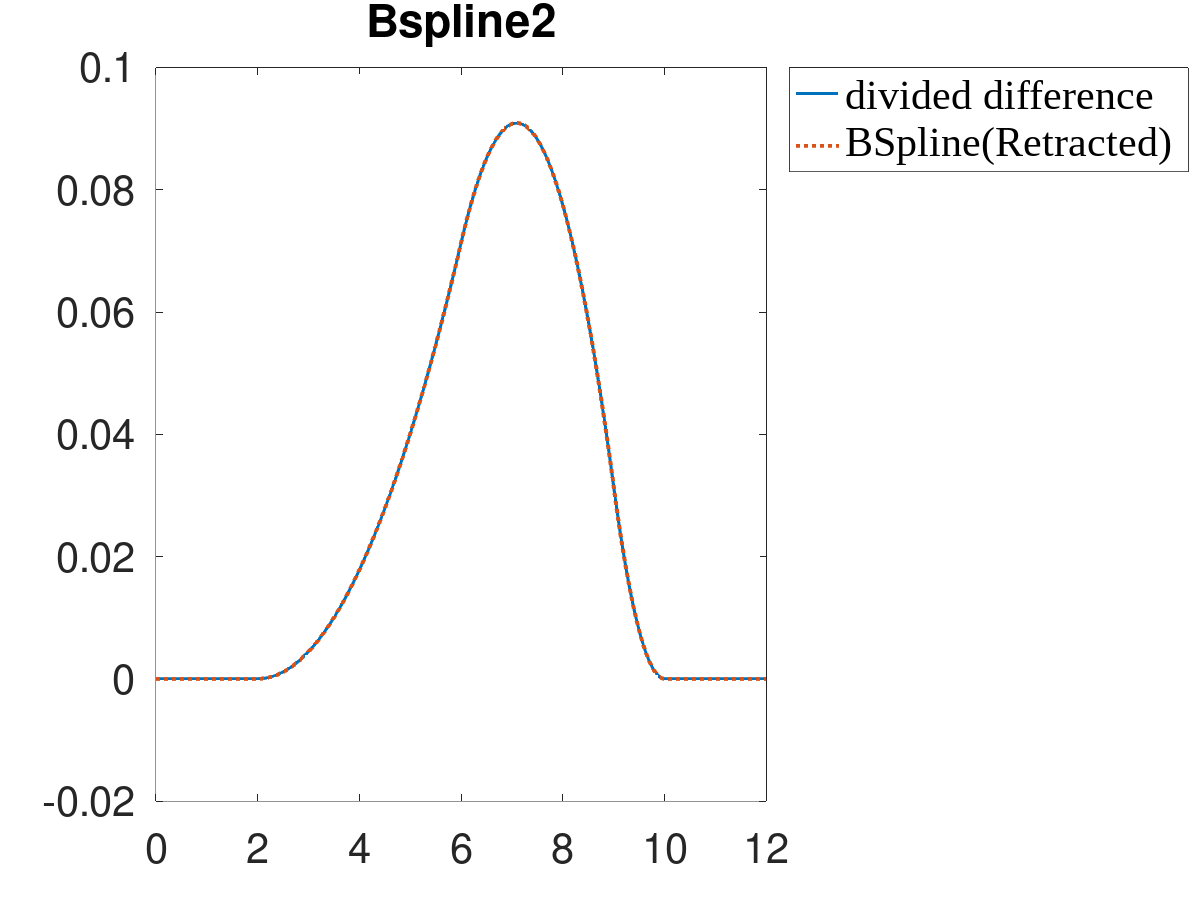
\includegraphics[width=0.45\textwidth]{figures/Assignment_G_2_Compare.png}

which corresponds to the theorem.

\end{document}
%%% Local Variables: 
%%% mode: latex
%%% TeX-master: t
%%% End: 
